%\documentclass[12pt]{report}
\documentclass{book}
\usepackage[utf8]{inputenc}
\usepackage[draft]{graphicx}
%\usepackage{graphicx}
\usepackage{amsmath}
\usepackage{physics}
\usepackage[noBBpl]{mathpazo}
%\usepackage{geometry} \geometry{ a4paper, total={170mm,257mm}, left=20mm, top=20mm,}
%\usepackage{geometry} \geometry{ a4paper, total={170mm,257mm}, left=30mm, right=30mm,}
\usepackage[space]{grffile}
\usepackage{amssymb}
\usepackage{hyperref}	
\usepackage[stable]{footmisc}
\usepackage{amssymb}
\usepackage[nottoc,numbib]{tocbibind}
\usepackage{dsfont}
\usepackage{framed}
%\usepackage[font=small,labelfont=bf]{caption}
\usepackage[font=small]{caption}
\usepackage{subcaption}
\usepackage{wrapfig}
\usepackage{bm}
\usepackage{siunitx}
\usepackage{floatrow}



\usepackage{xcolor}

\newcommand{\highlight}[1]{%
  \colorbox{green!30}{$\displaystyle#1$}}


\usepackage{newfloat}
\DeclareFloatingEnvironment[placement={!ht},name=List]{mylist}

\newcommand{\eff}{\text{eff}}
\newcommand*\Diff[1]{\mathop{}\!\mathrm{d^#1}}
\newcommand{\ncl}{\hat{a}\left(\hat{a}^\dagger \hat{a} - 1\right)}
\newcommand{\gncl}{\gamma_{\text{NCL}}}
\newcommand{\hc}{\text{h. c.}}
%\newcommand{\d}{\delta}
\newcommand*\erfc{\text{erfc}}
\newcommand{\perr}{\text{p}_{\text{err}}}
\newcommand{\perrps}{\perr\left(\Delta_r, \Delta_\theta\right)}
\newcommand{\pe}{\text{p}_{\text{e}}}
\newcommand{\given}{\; \middle| \;}
\newcommand{\cond}{\; | \;}
\newcommand{\tmsv}{\rho_{\text{TMSV}}}
\newcommand{\rps}{\mathcal{R}_{\text{PS}}}
\newcommand{{\systemB}}{QDS-$b$-QSS-$b$-CV-QPSK}
\newcommand{{\systemF}}{QDS-$f$-QKD-$f$-CV-QPSK}
\newcommand{\ddt}[1][]{\frac{\mathrm{d}#1}{\mathrm{d}t}}
\newcommand{\dims}{\left|\mathcal{H}\right|}
\newcommand{\code}[1]{\texttt{#1}}



\includeonly{
	%chapters/introduction,
	%chapters/crypto_intro,
%	chapters/qds,
%	chapters/qss,
%	chapters/aqc,
%	chapters/phog,
%	chapters/phog_adiabatic_elimination,
	chapters/phog_numerical_methods
}



%\DeclareGraphicsExtensions{.pdf,.png,.jpg}
\DeclareGraphicsExtensions{.png, .pdf,.jpg}


\usepackage{color} 
\def\red#1{\textcolor{red}{#1}}
\def\blue#1{\textcolor{blue}{#1}}
\def\MT#1{\textcolor{magenta}{#1}}
\def\cyan#1{\textcolor{cyan}{#1}}

\graphicspath{ {images/} }

\setcounter{tocdepth}{1} % Show sections
%\setcounter{tocdepth}{2} % + subsections
%\setcounter{tocdepth}{3} % + subsubsections
%\setcounter{tocdepth}{4} % + paragraphs
%\setcounter{tocdepth}{5} % + subparagraphs

%\title{Thesis draft - selected chapters}
%\date{\today}

\begin{document}
%\maketitle
%\tableofcontents

%\part{Secure quantum networks}


%\listoffigures
%\chapter{Introduction}

\subsection{Things to include}
\begin{itemize}
\item Beamsplitter properties and relations
\item Definitions and interpretations of various entropic quantities
\item Holevo information
\item Phase space
\item Background quantum mechanics
\item POVMs
\item Covariance matrices
\item Master equations
\item Coherent states
\item Homodyning and heterodyning
\item Mixed states, entangled states
\item Thermal state
\item TMSV state
\end{itemize}

\subsection{Hoeffding's inequalities}
Let $\mathcal{X} = X_1, X_2, \dots, X_n$ be $n$ independent binary random variables. Let $\bar{\mathcal{X}}$ be their empirical mean \MT{define} and let $\mathbb{E}\left(\bar{\mathcal{X}}\right)$ be its expected value. Then $\forall \epsilon \ge 0$ we may bound the probability that the empirical mean $\bar{\mathcal{X}}$ differs from its expectation $\mathbb{E}\left(\bar{\mathcal{X}}\right)$ by the following inequalities

\begin{align}
\label{eqn:hoeffding1}
\text{P}\left(\bar{\mathcal{X}} - \mathbb{E}\left(\bar{\mathcal{X}}\right) \ge \epsilon\right) &\le \text{exp}\left(- 2 \epsilon^2 n\right) \\
\label{eqn:hoeffding2}
\text{P}\left(\mathbb{E}\left(\bar{\mathcal{X}}\right) - \bar{\mathcal{X}} \ge \epsilon\right) &\le \text{exp}\left(- 2 \epsilon^2 n\right).
\end{align}

\noindent These inequalities are known as Hoeffding's inequalities \MT{cite} and will provide a necessary tool for analysis of our Quantum Digital Signatures protocol.


%\part{Agile cryptography: signatures and secrets}
%\chapter{Introduction to quantum cryptography}

\section{Conventional (classical) cryptography}
%introduction and literature review
Goal of chapter: historical overview of development of quantum cryptography. Lead up to a thorough literature review for QDS, QSS and QKD.

Cryptography is a field probably as old as civilization itself. For as long as communication has existed, so too has the desire to keep information hidden. Both the Greeks and the Romans are known to have used ciphers to encrypt messages \MT{cite}. A cipher, after applied to a message, alows the encrypted message to be freely transmitted and intercepted without an adverse party knowing its meaning. The intended recipients, however, can undo the effects of the cipher and read the original message. \MT{It'd be cool to have an example of e.g. a ceasar cipher}.

Cryptanalysis--the art and science of breaking cryptographic systems--has existed for as long as cryptography. The history of cryptographic development can be viewed as a race between cryptographers and cryptanalysts. The cryptographers, Alice and Bob, continually invent new schemes to perform their secure communication task. The cryptanalyst, Eve, continually tries to break these schemes in order to interfere in Alice and Bob's communication.

\MT{The following segue seems quite abrupt}
There are two main important strands of cryptography: private-key and public-key crytography, Fig.~\ref{fig:pubpriv}. In private-key cryptography (also known as \emph{symmetric} cryptography), Alice and Bob share some secret information which they will use to perform some task, and without which an eavesdropper cannot break the system. An important example of private-key cryptography is encryption with a cipher $\mathcal{K}$ which is used to encrypt and decrypt messages. Any party with $\mathcal{K}$ can freely encypt or decrypt any piece of information, while any party lacking knowledge of $\mathcal{K}$ cannot. A relevant example of this type of cryptosystem is the one-time pad (OTP) which is discussed above.

\MT{Perhaps some discussion about how $\mathcal{K}$ can be distributed and attacked}

\MT{I should have a discussion at some point about how public- and private- key cryptography relate to each other and how they are both used in modern infrastructure}

The second strand is public-key cryptography (also known as \emph{asymmetric} cryptography). Here, there are several pieces of information required to run a protocol. Alice is assumed to hold a key $\mathcal{E}$ (her ``private key'') while Bob holds a key $\mathcal{D}$ (Alice's ``public-key'') which is assumed to be publicly known. As an example, Alice may encrypt a message using $\mathcal{E}$ and sends it to Bob, who may decrypt it using $\mathcal{D}$.  \MT{Include more examples of this thing actually being used in practice}

\begin{figure}[htp]
\centering
\captionsetup{width=0.8\linewidth}
\begin{framed}
\begin{subfigure}{0.4\textwidth}
\begin{align*}
m \mapsto \text{Encrypt}_\mathcal{K}\left(m\right) \\
\text{Decrypt}_\mathcal{K}\left[E_\mathcal{K}\left(m\right)\right] \mapsto m
\end{align*}
\caption{}
\end{subfigure}
\begin{subfigure}{0.4\textwidth}
\begin{align*}
m \mapsto \text{Encrypt}_\mathcal{E}\left(m\right) \\
\text{Decrypt}_\mathcal{D}\left[\text{Encrypt}_\mathcal{E}\left(m\right)\right] \mapsto m
\end{align*}
\caption{}
\end{subfigure}
\caption{(a) Private-key encryption. The same key $\mathcal{K}$ allows Alice to encrypt and Bob to decrypt message $m$. (b) Public-key encryption. Alice and Bob use different keys, $\mathcal{E}$ and $\mathcal{D}$ to encrypt and decrypt $m$. The decyption key $\mathcal{D}$ can be public knowledge without affecting the security of the encryption key $\mathcal{E}$.}
\label{fig:pubpriv}
\end{framed}
\end{figure}

Usually, given knowledge of $\mathcal{E}$ it should be easy to derive $\mathcal{D}$. The converse should not be true, and the publicly available $\mathcal{D}$ should give no indication of $\mathcal{E}$. If $\mathcal{E}$ is unique to Alice, then a successful decryption using $\mathcal{D}$ proves sufficient to prove Alice's identity.\footnote{One may be tempted to build a digital signatures protocol on this exchange, but \MT{explain why it is a bad idea, with reference to Simmons}.}

The function $f: \mathcal{E} \mapsto \mathcal{D}$ is sometimes referred to as a ``trapdoor'' or ``one-way'' function, and $f$ is typically based on a mathematical problem which is deemed to be computationally hard, for example \MT{examples} which underly the commonly used \MT{protocols}. \MT{motivate quantum cryptography via breaking of these trapdoors}


\section{Quantum digital signatures protocols}
%This section will basically be my "literature review" section.
%I will focus on the main thread of QDS developments initially, but I can supplement it by including some of the asian papers later.

%Note: after I have this section I can compare it to the Amiri2015 review paper and to Collins2018 progress report (and to Callum's thesis)


\subsection*{Quantum one-way function}
%Talk about Gottesman and Chuang.
Gottesman and Chuang \cite{Gottesman2001} generalized Lamport's scheme \MT{cite} in $2001$ to build the first Quantum Digital Signatures protocol. The key contribution of their scheme is to replace the one-way function in \MT{cite} with a so-called \emph{quantum one-way function}, thereby securing the signatures protocol against a quantum adversary.

\MT{TODO: chat more about quantum one-way function. Include the "figure" that I currently have in my historical introduction}

A direct analogue of public-key cryptography, their protocol relies on the difficult task, described in Fig.~\MT{X}, of accurately distinguishing between non-orthogonal quantum states. Their security relies on the fact that performing measurement on a state of $n$~qubits can yield at most $n$~bits of information, and so the protocol in Ref.~\cite{Gottesman2001} is designed such that this is insufficient to distinguish between states.

The key tool in the protocol is a quantum $SWAP$ test, Fig.~\MT{X}, which probabilistically determines whether two states are identical. To perform this test, players prepare $\ket{f_x}, \ket{f_{x^\prime}}$ and an additional ancilla $\left(\ket{0} + \ket{1}\right)/\sqrt{2}$. Players perform a Fredkin gate \MT{cite} using the ancilla as a control, and then perform a Hadamard \MT{cite} on the ancilla. In other words, the $SWAP$ test performs the mapping
\begin{equation}
\ket{f_x}\ket{f_{x^\prime}}\frac{\left(\ket{0} + \ket{1}\right)}{\sqrt{2}} \mapsto \frac{\left(\ket{f_x}\ket{f_{x^\prime}} \pm \ket{f_{x^\prime}}\ket{f_x}\right)\ket{y_{\pm}}}{\sqrt{2}}
\end{equation}
with $y_+=0$ and $y_-=1$. Finally, the ancilla qubit is measured in the $0, 1$ basis, and since $\ket{0}, \ket{1}$ are orthogonal they can be distinguished.  Therefore if $x = x^\prime$ the coefficient of $\ket{1}$ is identically zero, and so the $SWAP$ test always outputs $\ket{0}$. If $x \ne x^\prime$ outputs either $\ket{1}$ or $\ket{0}$. 

The probabilistic nature of this test will cause participants in the protocol to sometimes mistake distinct states for identical ones, but the probability that this occurs may be estimated. Crucially, the protocol may be proven secure if states are chosen such that this probability of honest failure is smaller than the probability to correctly distinguish between large entangled states of non-orthogonal qubits. 

The protocol is a significant attempt to generalise and translate structures from the field of classical cryptography to the quantum realm, and it sets the pattern for all subsequent QDS protocols, and so it is worth examining the protocol in detail. Alice has a $1$~bit message $b$ which she would like to sign, and send to Bob and Charlie. In the Distribution state, for each $b$ Alice creates $M$ classical strings $k_m^i$, length $L$. Each classical string is mapped to a corresponding quantum state $\ket{k_m^i}$ of $n$~qubits which are chosen to be highly non-orthogonal. Two of each of these quantum states are sent to Bob and Charlie. The quantum states, $4M$ in total, are Alice's public keys which may be freely distributed--and they may even be given to a dishonest external party. The corresponding classical strings $k_m^i$ are Alice's private keys.

Bob and Charlie each receive two of the $\ket{k_m^i}$. They each perform a $SWAP$ test between their two copies of the public key, to check whether individual copies are equivalent. Then, they should perform a $SWAP$ test between one of Bob's keys and one of Charlie's keys, to test whether they received identical keys to each other. If all $SWAP$ tests pass then the protocol continues to the next step, otherwise it aborts. Bob and Charlie should now store the quantum public keys which they hold.

Later, in the Messaging stage, Alice sends $\left(m, k_m^i\right)$. For each of the $M$ strings $k_m^i$, Bob creates $\ket{k_m^i}$ and performs a $SWAP$ test with his corresponding stored quantum state. If his test passes most of the time then he accepts the message as genuine and transferable, and passes $\left(m, k_m^i\right)$ to Charlie who performs similar tests. 

Although laying the groundwork for practical QDS protocols, this original proposal cannot be implemented. The most pressing problem is the requirement for long-term quantum memory. State-of-the-art technology can store a quantum state for \MT{X}, and so long-term storage of many copies of quantum states with many qubits will be technologically challenging. Furthermore, the need for every party to be able to create and distribute the states and the multiple required $SWAP$ tests render this protocol impractical for implementation. 

However, as we shall see, the structure of this protocol is very closely aligned to classical signatures protocols. Since the public keys are truly public (all of them can be handed to Eve). Furthermore, every recipient is given identical quantum public keys and so the number of recipients does not need to be fixed before the start of the protocol. These requirements are subtly changed in later--more practical--QDS protocols. \MT{make sure I talk about this later.}

\MT{Perhaps talk about repudiation somewhere in this section?}

%\subsection{Andersson2006 (+ implementation)}
\subsection*{QDS implementation}
%Talk about Andersson2006 and Clarke2012

%\subsection{Dunjko2014 (+ implementation}
\subsection*{Removing quantum memory}
The requirement that recipients possess long-term and efficient quantum memory, needed for the above protocol, makes it impractical for realization. The removal of this requirement by Dunjko \emph{et. al.} \cite{Dunjko2014} was one of the major milestones towards a practical QDS which can be implemented. 

The key insight of Ref.~\cite{Dunjko2014} was to effectively replace the quantum public key by a classical one, albeit one which relies on the distribution and measurement of non-orthogonal quantum states. This physical requirement is a practical one, relying on simply linear optics (beamsplitters) and photodetectors capable of distinguishing just between zero and nonzero photon numbers. The storage of classical public keys is clearly no restriction. 

The main difference then between Refs.~\cite{Dunjko2014} and \cite{Gottesman2001}, is that in Dunjko \emph{et. al.}, recipients Bob and Charlie perform photon-number measurement as they receive the quantum states. Remarkably, despite this fundamental change to the nature of the protocol's one-way function, secure QDS is possible. \MT{do I need to revise this sentence? Is it accurate and fair?}

\MT{Include a figure (minipage thing) comparing the one-way functions used by Gottesman2001 and by Dunjko2014.}

In the Distribution stage of the protocol, Alice generates classical strings $\left\{k_j^m\right\}_{j=0}^L$, length $L$, corresponding to each future one-bit message $m$. The $k_j^m$ are chosen uniformly at random from the BPSK alphabet of coherent state phases $\left\{- \alpha, \alpha\right\}$. Alice then forms sequences of coherent states $\rho = \otimes_{j=0}^L \ket{k_j^m}$ which she then distributes to Bob and to Charlie. 

\begin{figure}[htp]
\centering
\includegraphics[width=0.8\linewidth]{multiport.png}
\caption{\label{fig:dunjko2014_multiport}}
\end{figure}

Bob and Charlie pass their received coherent states through the shared optical multiport, Fig.~\ref{fig:dunjko2014_multiport}, which serves to symmetrize their individual quantum states. That is, after the multiport Bob and Charlie's reduced density matrices are identical, which guards against Alice's repudiation attack. Each recipient has two outputs of the multiport. One output, the so-called "null-port" should be monitored for clicks of the photodiode which imply that $\alpha \ne \beta$ (Bob and Charlie have different coherent states, Fig.~\ref{fig:dunjko2014_multiport}) which may imply the presence of an attack. Bob and Charlie should also perform unambiguous state discrimination (USD) on the outputs of their signal ports, which will accurately distinguish between non-orthogonal states $\ket{\alpha}, \ket{-\alpha}$ at the expense that it will sometimes fail to give an answer. 

During Messaging, Alice will declare $\left(m, k_j^m\right)$ which recipients will compare to their USD outcomes. Provided that there are enough matches between Alice's phase declarations $k_j^m$ and Bob/Charlie's USD outcomes, message $m$ is accepted and the protocol has succeeded.

This first protocol avoiding the requirement for quantum memory shows that QDS may be both practical and secure. Furthermore the limited physical requirements--tensor-products of coherent states, beamsplitters and non-photon-number-resolving detectors--are feasible to work with, unlike the large number of superposition qubits required for Ref.~\cite{Gottesman2001}. \MT{Now talk about the implementation paper}.

Notice though the subtle shift between Refs.~\cite{Gottesman2001} and \cite{Dunjko2014}. While previously the number of recipients did not need to be determined until the Messaging stage, here it must be determined before Distribution. After the coherent states have passed through the multiport the number of recipients cannot be changed. 
\MT{I should note later that removing the multiport removes this restriction.} Because of the physical requirement for the optical multiport, it will also be challenging (though possible) to generalize to more recipients, at the expense of altering the protocol to rely on a measurement scheme other than USD. \MT{why?}. Realistic implementation of the multiport also introduces noise and losses due to misalignment and instability, further reducing the efficiency of the protocol.


The most difficult assumption which Ref.~\cite{Dunjko2014} makes, however, is that there should be no eavesdroppers on the quantum channels. This is a strong and impractical assumption, and one which subsequent papers will endeavour to remove.







\subsection{Wallden2015 (+ implementation)}

\subsection{Tokyo installed fibers scheme}
\MT{Perhaps the rest of the DPS-based protocols here too?}

\subsection{Amiri2016 (+ implementation)}

\subsection{Puthoor2016 (+ implementation)}
\MT{Though first talk about side-channel attacks}

\subsection{The other "almost-agile" ones?}

\subsection{An2019 (+ implementation)}

\subsection{Croal2016}
\MT{Discuss DV vs CV first}

\subsection{Quick chat about my PRA}

\subsection{"Classical" unconditionally secure signatures}

\subsection{Extensions to signature schemes}

\MT{then I can have a section on QSS lit review and introduction, and one for agility. This way the chapters can be shorter and more readable.}
%\section{Quantum digital signatures protocols}
%This section will basically be my "literature review" section.
%I will focus on the main thread of QDS developments initially, but I can supplement it by including some of the asian papers later.

%Note: after I have this section I can compare it to the Amiri2015 review paper and to Collins2018 progress report (and to Callum's thesis)


\subsection*{Quantum one-way function}
%Talk about Gottesman and Chuang.
Gottesman and Chuang \cite{Gottesman2001} generalized Lamport's scheme \MT{cite} in $2001$ to build the first Quantum Digital Signatures protocol. The key contribution of their scheme is to replace the one-way function in \MT{cite} with a so-called \emph{quantum one-way function}, thereby securing the signatures protocol against a quantum adversary.

\MT{TODO: chat more about quantum one-way function. Include the "figure" that I currently have in my historical introduction}

A direct analogue of public-key cryptography, their protocol relies on the difficult task, described in Fig.~\MT{X}, of accurately distinguishing between non-orthogonal quantum states. Their security relies on the fact that performing measurement on a state of $n$~qubits can yield at most $n$~bits of information, and so the protocol in Ref.~\cite{Gottesman2001} is designed such that this is insufficient to distinguish between states.

The key tool in the protocol is a quantum $SWAP$ test, Fig.~\MT{X}, which probabilistically determines whether two states are identical. To perform this test, players prepare $\ket{f_x}, \ket{f_{x^\prime}}$ and an additional ancilla $\left(\ket{0} + \ket{1}\right)/\sqrt{2}$. Players perform a Fredkin gate \MT{cite} using the ancilla as a control, and then perform a Hadamard \MT{cite} on the ancilla. In other words, the $SWAP$ test performs the mapping
\begin{equation}
\ket{f_x}\ket{f_{x^\prime}}\frac{\left(\ket{0} + \ket{1}\right)}{\sqrt{2}} \mapsto \frac{\left(\ket{f_x}\ket{f_{x^\prime}} \pm \ket{f_{x^\prime}}\ket{f_x}\right)\ket{y_{\pm}}}{\sqrt{2}}
\end{equation}
with $y_+=0$ and $y_-=1$. Finally, the ancilla qubit is measured in the $0, 1$ basis, and since $\ket{0}, \ket{1}$ are orthogonal they can be distinguished.  Therefore if $x = x^\prime$ the coefficient of $\ket{1}$ is identically zero, and so the $SWAP$ test always outputs $\ket{0}$. If $x \ne x^\prime$ outputs either $\ket{1}$ or $\ket{0}$. 

The probabilistic nature of this test will cause participants in the protocol to sometimes mistake distinct states for identical ones, but the probability that this occurs may be estimated. Crucially, the protocol may be proven secure if states are chosen such that this probability of honest failure is smaller than the probability to correctly distinguish between large entangled states of non-orthogonal qubits. 

The protocol is a significant attempt to generalise and translate structures from the field of classical cryptography to the quantum realm, and it sets the pattern for all subsequent QDS protocols, and so it is worth examining the protocol in detail. Alice has a $1$~bit message $b$ which she would like to sign, and send to Bob and Charlie. In the Distribution state, for each $b$ Alice creates $M$ classical strings $k_m^i$, length $L$. Each classical string is mapped to a corresponding quantum state $\ket{k_m^i}$ of $n$~qubits which are chosen to be highly non-orthogonal. Two of each of these quantum states are sent to Bob and Charlie. The quantum states, $4M$ in total, are Alice's public keys which may be freely distributed--and they may even be given to a dishonest external party. The corresponding classical strings $k_m^i$ are Alice's private keys.

Bob and Charlie each receive two of the $\ket{k_m^i}$. They each perform a $SWAP$ test between their two copies of the public key, to check whether individual copies are equivalent. Then, they should perform a $SWAP$ test between one of Bob's keys and one of Charlie's keys, to test whether they received identical keys to each other. If all $SWAP$ tests pass then the protocol continues to the next step, otherwise it aborts. Bob and Charlie should now store the quantum public keys which they hold.

Later, in the Messaging stage, Alice sends $\left(m, k_m^i\right)$. For each of the $M$ strings $k_m^i$, Bob creates $\ket{k_m^i}$ and performs a $SWAP$ test with his corresponding stored quantum state. If his test passes most of the time then he accepts the message as genuine and transferable, and passes $\left(m, k_m^i\right)$ to Charlie who performs similar tests. 

Although laying the groundwork for practical QDS protocols, this original proposal cannot be implemented. The most pressing problem is the requirement for long-term quantum memory. State-of-the-art technology can store a quantum state for \MT{X}, and so long-term storage of many copies of quantum states with many qubits will be technologically challenging. Furthermore, the need for every party to be able to create and distribute the states and the multiple required $SWAP$ tests render this protocol impractical for implementation. 

However, as we shall see, the structure of this protocol is very closely aligned to classical signatures protocols. Since the public keys are truly public (all of them can be handed to Eve). Furthermore, every recipient is given identical quantum public keys and so the number of recipients does not need to be fixed before the start of the protocol. These requirements are subtly changed in later--more practical--QDS protocols. \MT{make sure I talk about this later.}

\MT{Perhaps talk about repudiation somewhere in this section?}

%\subsection{Andersson2006 (+ implementation)}
\subsection*{QDS implementation}
%Talk about Andersson2006 and Clarke2012

%\subsection{Dunjko2014 (+ implementation}
\subsection*{Removing quantum memory}
The requirement that recipients possess long-term and efficient quantum memory, needed for the above protocol, makes it impractical for realization. The removal of this requirement by Dunjko \emph{et. al.} \cite{Dunjko2014} was one of the major milestones towards a practical QDS which can be implemented. 

The key insight of Ref.~\cite{Dunjko2014} was to effectively replace the quantum public key by a classical one, albeit one which relies on the distribution and measurement of non-orthogonal quantum states. This physical requirement is a practical one, relying on simply linear optics (beamsplitters) and photodetectors capable of distinguishing just between zero and nonzero photon numbers. The storage of classical public keys is clearly no restriction. 

The main difference then between Refs.~\cite{Dunjko2014} and \cite{Gottesman2001}, is that in Dunjko \emph{et. al.}, recipients Bob and Charlie perform photon-number measurement as they receive the quantum states. Remarkably, despite this fundamental change to the nature of the protocol's one-way function, secure QDS is possible. \MT{do I need to revise this sentence? Is it accurate and fair?}

\MT{Include a figure (minipage thing) comparing the one-way functions used by Gottesman2001 and by Dunjko2014.}

In the Distribution stage of the protocol, Alice generates classical strings $\left\{k_j^m\right\}_{j=0}^L$, length $L$, corresponding to each future one-bit message $m$. The $k_j^m$ are chosen uniformly at random from the BPSK alphabet of coherent state phases $\left\{- \alpha, \alpha\right\}$. Alice then forms sequences of coherent states $\rho = \otimes_{j=0}^L \ket{k_j^m}$ which she then distributes to Bob and to Charlie. 

\begin{figure}[htp]
\centering
\includegraphics[width=0.8\linewidth]{multiport.png}
\caption{\label{fig:dunjko2014_multiport}}
\end{figure}

Bob and Charlie pass their received coherent states through the shared optical multiport, Fig.~\ref{fig:dunjko2014_multiport}, which serves to symmetrize their individual quantum states. That is, after the multiport Bob and Charlie's reduced density matrices are identical, which guards against Alice's repudiation attack. Each recipient has two outputs of the multiport. One output, the so-called "null-port" should be monitored for clicks of the photodiode which imply that $\alpha \ne \beta$ (Bob and Charlie have different coherent states, Fig.~\ref{fig:dunjko2014_multiport}) which may imply the presence of an attack. Bob and Charlie should also perform unambiguous state discrimination (USD) on the outputs of their signal ports, which will accurately distinguish between non-orthogonal states $\ket{\alpha}, \ket{-\alpha}$ at the expense that it will sometimes fail to give an answer. 

During Messaging, Alice will declare $\left(m, k_j^m\right)$ which recipients will compare to their USD outcomes. Provided that there are enough matches between Alice's phase declarations $k_j^m$ and Bob/Charlie's USD outcomes, message $m$ is accepted and the protocol has succeeded.

This first protocol avoiding the requirement for quantum memory shows that QDS may be both practical and secure. Furthermore the limited physical requirements--tensor-products of coherent states, beamsplitters and non-photon-number-resolving detectors--are feasible to work with, unlike the large number of superposition qubits required for Ref.~\cite{Gottesman2001}. \MT{Now talk about the implementation paper}.

Notice though the subtle shift between Refs.~\cite{Gottesman2001} and \cite{Dunjko2014}. While previously the number of recipients did not need to be determined until the Messaging stage, here it must be determined before Distribution. After the coherent states have passed through the multiport the number of recipients cannot be changed. 
\MT{I should note later that removing the multiport removes this restriction.} Because of the physical requirement for the optical multiport, it will also be challenging (though possible) to generalize to more recipients, at the expense of altering the protocol to rely on a measurement scheme other than USD. \MT{why?}. Realistic implementation of the multiport also introduces noise and losses due to misalignment and instability, further reducing the efficiency of the protocol.


The most difficult assumption which Ref.~\cite{Dunjko2014} makes, however, is that there should be no eavesdroppers on the quantum channels. This is a strong and impractical assumption, and one which subsequent papers will endeavour to remove.







\subsection{Wallden2015 (+ implementation)}

\subsection{Tokyo installed fibers scheme}
\MT{Perhaps the rest of the DPS-based protocols here too?}

\subsection{Amiri2016 (+ implementation)}

\subsection{Puthoor2016 (+ implementation)}
\MT{Though first talk about side-channel attacks}

\subsection{The other "almost-agile" ones?}

\subsection{An2019 (+ implementation)}

\subsection{Croal2016}
\MT{Discuss DV vs CV first}

\subsection{Quick chat about my PRA}

\subsection{"Classical" unconditionally secure signatures}

\subsection{Extensions to signature schemes}
%\chapter{Quantum digital signatures}
Goal of chapter: introduce our QDS protocol and prove its security in different contexts using several methods.

\section{QDS protocol description}

In the simplest instance we may consider the signaure scheme involving only three parties: a sender, Alice ($A$), and recipients Bob ($B$) and Charlie ($C$). Alice wishes to send a classical message $m$ to $B$ and $C$, such that $B$ and $C$ can correctly determine whether $m$ was indeed sent by $A$. Furthermore the recipients should be able to check whether $m$ has been altered.

\subsection{Goals of a signature scheme}
\MT{Add introduction, and chat about how the multipartite setting is actually quite interesting}

A digital signature scheme must ensure that the following requirements are fulfilled:

\noindent \emph{$1$. Security against forgery}: Neither a dishonest recipient ($B$ or $C$), nor an external fourth party (Eve, $E$), should be able to alter $m$ and have it accepted as genuine by an honest recipient. That is, the signature scheme should ensure that $m$ is the message which Alice sent.

\noindent \emph{$2$. Genuine sender}: Neither a dishonest recipient ($B$ or $C$), nor an external fourth party (Eve, $E$), should be able to impersonate $A$. A message which falsely claims to have originated with Alice should be rejected.

\noindent \emph{$3$. Security against repudiation}: A dishonest sender $A$ should not be able to cause disagreement between $B$, $C$ about the previous two requirements. That is, after genuinely sending $m$ she should not later be able to deny it. If Bob accepts the message as genuine then so too should Charlie. 

\noindent \emph{$4$. Message transferability}: If $B$ accepts a message as genuine, then so too should $C$. In the simple $3$~party signatures protocol considered here, this requirement is equivalent to requirement $3$, while when more recipients are involved one may define a message $m^{\left(k\right)}$ as $k$-transferable if it can be successfully forwarded up to $k$ times. That is, if recipient $B_0$ accepts $m^{\left(k\right)}$, then recipients $B_1 \dots B_k$ should also accept.

For our scheme involving three parties (only two recipients), requirements $3$ and $4$ are equivalent, and so in what follows we will talk about repudiation only. Requirements $1$ and $2$ are fulfilled in our scheme by the same security process, and so we will focus on $1$ and simply note where $2$ arises.

\MT{Let's have a nice figure explaining each of these attacks, similar to the one from my CEWQO2018 poster, but without proprietary content}

A digital signature scheme which rejects all messages trivially fulfills requirements $1-4$, and so in order to get a useful digital signature scheme we impose:

\noindent \emph{$5$. Robustness}: In the absence of $E$, the message $m$ should be accepted if $A, B, C$ behave honestly.

\subsection{Our QDS scheme}

We here present a continuous-variable (CV) QDS protocol based on the quadrature phase-shift keying (QPSK) alphabet of coherent states. %this will be defined earlier, I am sure
Our protocol allows us to take into account quantum distribution channels which will in general be insecure, and this scheme is the first in the CV setting to be secure against eavesdropping. \MT{I should motivate the CV setting somewhere, probably in ch1}

Our QDS scheme is split into two stages, Distribution and Messaging, which can occur with significant time delay. The quantum states are sent and measured during Distribution, while during Messaging Alice will send her message and classical signature, and Bob and Charlie will try to determine its validity.\footnote{Note the intrinsic separation between the Distribution (quantum) and Messaging (classical) stages of the protocol. We will take further advantage of this separation between quantum and classical steps in Chapter~\MT{X}} Our protocol setup is outlined in Fig.~\MT{X}, while the protocol is described in Fig.~\MT{X} % I want a flowchart-style figure to outline the steps of the protocol

\MT{mention somewhere why we consider just a $1$ bit message}

\MT{I'll do everything for QPSK, but I should have a section where I generalize to NPSK}

\subsubsection{Distribution stage}
\noindent Step $1$. Alice wishes to send a signed $1$ bit message $m$ to Bob and Charlie. For each possible future $m$, and for each recipient, Alice creates the following classical strings
\begin{equation}
\Phi_m^{\left(B, C\right)} = \left\{ \phi_{j, m}^{\left(B, C\right)\right\}_{j=1}^{L}
\end{equation}
where the $phi_{j}$ are complex phases chosen from alphabet $\mathcal{A}_4$. The signature length $L$ is an integer suitably chosen to ensure the desired level of security.

















%%%
%
% TODO:
% - talk somewhere about the types of attack which we allow
% - make sure I talk about the types of channel which we use
% Q: where should I talk about Alice's function F?
% - understand the mapping from complex values to binary
% - some more remarks about the running of the protocol?
% - mention somewhere my linestyle convention for different types of channel

\chapter{Quantum secret sharing}
Goal of chapter: introduce our QSS protocol and prove its security in different contexts.

\iffalse
Key results which I want to present:
\begin{itemize}
\item our QSS protocol
\item security proof (what does it do? what does it not do?)
\item analysis of security in various settings - heterodyne, $\mathcal{A}_4$, BS0, BS1, BS2, EC, varying $\alpha$, $T$, $\xi$, $g$, $h$ of both channels
\item show how the protocol performs
\end{itemize}
\fi

\MT{Short introduction to chapter.}

\section{Our QSS protocol}

Our quantum secret-sharing scheme allows for a dealer, Alice, to distribute a classical secret between two recipients, Bob and Charlie. Bob and Charlie should be able to exactly reconstruct the secret when they behave honestly, while a dishonest and unauthorised conspiracy of players--including those outside the protocol--should gain no information. Crucially, although the scheme should allow for dishonesty among the recipients a dishonest player should be forced to collaborate with an honest one.

\begin{figure}[htp]
\centering
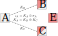
\includegraphics[draft=false, width=0.5\linewidth]{qss/qss_setup_cartoon}
\caption{\label{fig:qss_structure} All quantum secret sharing schemes follow the same structure. Alice encrypts her classical secret $\sigma_A$ with key $K_A$, and broadcasts the resulting $\varsigma_A$. Shares of $K_A$ are distributed among recipients Bob and Charlie such that $K_B \oplus K_C = K_A$. Gray boxes denote honest players, while red denotes dishonest players. The half-red/half-gray boxes denote uncertainty about which player is dishonest. %say somewhere it's all classical?
}
\end{figure}

\subsection{QSS setup}

All QSS protocols follow essentially the same structure, Fig.~\ref{fig:qss_structure}:
\begin{enumerate}
\item Alice (A) uses quantum resources to distribute shares of classical key $K_A$ among recipients Bob (B) and Charlie (C), such that $K_A = K_B \oplus K_C$.
\item Alice encrypts her secret $\varsigma_A = K_A \oplus \sigma_A$ and makes the encrypted secret $\varsigma_A$ publicly known.
\end{enumerate}
The $\oplus$ operation corresponds to bitwise addition (XOR) of binary keys and, provided that $K_A, K_B, K_C$ and $\sigma_A$ are the same length, the above secret sharing operation is provably unconditionally secure \cite{Schneier1996}, provided that key shares $K_B, K_C$ are securely distributed.

This form is similar to QKD-based encryption and it is for this reason that renowned cryptographer Gustavus Simmons wrote that 

\begin{center}\emph{``Secret sharing is simply a special form of key distribution''}\end{center}

\noindent as the abstract to Ref.~\cite{Simmons1990a}.

QSS protocols then only differ in the method used to generate and share the $K_B, K_C$ forming the encryption key. One attractive option would be for Alice to perform individual QKD protocols, first with Bob and then with Charlie, and then XOR the resulting keys together. Since QKD is provably secure, neither Bob nor Charlie can gain sufficient information about the other player's key. The resulting QSS scheme is thus also secure. We discuss this form of QSS at length in Sec.~\ref{sec:intro_qss_lit_review} and again in Chapter~\cite{chapter:aqc}.

Other options for generation and distribution of $K_B, K_C$ are discussed in Sec.~\ref{sec:intro_qss_lit_review} and fall into one of two categories. The first category \cite{Hillery1999, Karlsson1999, Gottesman1999, Markham2008, Wu2016, Kogias2017} relies on large entangled states shared between all $N$ players, while the second category \cite{Zhang2005a, Schmid2005, Schmid2007, Grice2019}, involves distribution of a single (typically one-mode) quantum state between all $N$ players, who each perform their choice of measurement on the state. In both forms, if $N-1$ players communicate and share their choice of measurement and their measurement outcomes, they have sufficient information to infer the measurement outcome of the $N^{\text{th}}$ player. In this way, a key $K_A$ is distributed between players.


\subsection{QSS protocol description}

We propose a QSS protocol which will perform the task of quantum secret sharing without requiring the distribution of highly entangled states between players \cite{Kogias2017} and without requiring a dedicated hardware or network setup \cite{Grice2019}. Instead, we rely on distribution of QPSK alphabet Eq.~\ref{eqn:intro_qpsk} and heterodyne detection Sec.~\ref{eqn:intro_heterodyne}. The QSS protocol guards against both eavesdropping by choice of QPSK alphabet with small coherent state amplitude $\alpha$, which ensures that Eve cannot accurately guess Alice's heterodyne outcomes. The protocol guards against the internal dishonesty of Bob or Charlie by ensuring that the key $K_A$ which Alice will use to encrypt her secret is a function of \emph{both} Bob and Charlie's information.% The dishonest internal player is then forced to collaborate with Eve to attack the honest player's quantum channel, which, by our choice of alphabet, will not succeed.

In our protocol, Bob and Charlie are chosen as the senders of the quantum states. This has advantage in that we may fully trust Alice's heterodyne detection\footnote{Note that permitting Bob or Charlie to perform the heterodyne detection implicitly places trust in their heterodyning beamsplitter \cite{Walk2016a}.} and its characterisation. A dishonest internal player will be forced to collaborate with Eve to attack the honest player's quantum channel. By our choice of alphabet, this will not succeed.

\begin{figure}[htp]
\centering
	\begin{subfigure}{0.8\linewidth}
		\centering
		\caption{\label{fig:qss_distribution_stage}}
		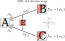
\includegraphics[draft=false, width=\linewidth]{qss/qss_distribution_stage}
		
	\end{subfigure}
	\begin{subfigure}{0.8\linewidth}
		\centering
		\caption{\label{fig:qss_encryption_stage}}
		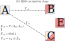
\includegraphics[draft=false, width=\linewidth]{qss/qss_encryption_stage}
		
	\end{subfigure}
\caption{\label{fig:qss_protocol_cartoon} Distribution and encryption stages of our QSS protocol. Alice (A) wishes to securely share her secret $\sigma_A$ amongst potentially dishonest recipients Bob (B) and Charlie (C). (a) Distribution stage. B and C send coherent states chosen from QPSK alphabet to Alice, who heterodynes and obtains outcomes $A_B, A_C$. Dishonest Eve will eavesdrop on the distribution of quantum states in order to gain information about $A_B, A_C$. (b) Encryption stage. Alice will form variable $X_A$ using her chosen function $\mathcal{F}$ with her heterodyne measurement outcomes as input variables. She converts $X_A$ to binary $\tilde{X}_A$ and encrypts the secret with it to reach $\varsigma_A = \sigma_A \oplus \tilde{X}_A$. The encrypted secret is then broadcast. Dishonest players are shown in red and honest players in gray. A combination of red and gray denotes uncertainty about dishonesty.
}
\end{figure}

Since Alice is the dealer who will decide on the eventual shared key our protocol is analogous to a reverse-reconciliation (RR) QKD system, and so we may similarly expect the performance benefits of RR QKD at high loss and noise. We note that having potentially untrusted players as the senders may open the protocol up to new classes of attack, for example if they are permitted to send a state which is outside the QPSK alphabet, and such attacks should be addressed in future work.

%\MT{talk somewhere about the types of attack we allow}


Our QSS protocol runs in three stages, a Distribution stage, an Encryption stage and, finally, a Decryption stage. Distribution and encryption stages are displayed in Fig.~\ref{fig:qss_protocol_cartoon}. The Distribution stage, Fig.~\ref{fig:qss_distribution_stage}, involves distribution and measurement of quantum coherent states chosen from QPSK alphabet. At the end of Distribution, Alice will hold classical information which is correlated with both Bob and Charlie. In the Encryption stage, Fig.~\ref{fig:qss_encryption_stage}, Alice will combine her classical information and use it to encode her sensitive classical secret. The encoded secret is distributed to Bob and Charlie. The secret is decoded by Bob and Charlie during Decryption. Our protocol setup is described in Fig.~\ref{fig:qss_structure},~\ref{fig:qss_protocol_cartoon}, and we describe it in detail below.

%\MT{make sure that the following is in the same style as my qds protocol description}

\subsubsection*{Distribution stage, Fig.~\ref{fig:qss_distribution_stage}}
\paragraph{Step $1$}
Alice wishes to encrypt a classical secret, $\sigma_A$. Bob forms a classical random variable $X_B = \left\{\phi_B\right\}$, where the $\phi_B$ are complex phases independently chosen from the QPSK alphabet. Phases $\phi_B$ are assumed to be chosen uniformly at random, but we relax this assumption in Chapter~\ref{chapter:aqc}. Charlie likewise forms classical random variable $X_C = \left\{\phi_C\right\}$.

\paragraph{Step $2$}
Bob and Charlie form sequences of coherent states based on their random variables
\begin{equation}
\rho\left[X_{\left(B, C\right)}\right] := \otimes \rho\left[\phi_{\left(B, C\right)}\right]
\end{equation}
where $\rho\left[\phi_{\left(B, C\right)}\right]$ denotes a coherent state with phase $\phi_{\left(B, C\right)}$. These sequences of states are sent to Alice through quantum channels. %\MT{Talk later about the types of channels which these are.}. 
Alice performs heterodyne detection, Sec.~\ref{sec:intro_heterodyne} on each of her received states and records her complex outcomes. We denote the strings of Alice's measurement outcomes as $A_B, A_C$, where $A_B$ corresponds to measurement outcomes from states sent by Bob, and $A_C$ corresponds to those on states sent by Charlie. The $A_B$ and $A_C$ are kept separate and secret, and Bob and Charlie should retain their information $X_B, X_C$.

\subsubsection*{Encryption stage, Fig.~\ref{fig:qss_encryption_stage}}

\paragraph{Step $3$} Alice creates a new string of complex variables
\begin{equation}
X_A = \mathcal{F}\left(A_B, A_C\right)
\end{equation}
from her measurement outcomes. The function $\mathcal{F}$ is chosen by Alice and should be freely chosen to optimize security. In this thesis we will pick simple forms for $\mathcal{F}$ which allow us to easily make concrete predictions about protocol security, although in general $\mathcal{F}$ may be as pathological as Alice desires.

% \MT{Where shall I talk about function $F$?} \MT{I can create some nice graphs of different functions $F$, even those requiring a lot of parameters to be optimized over. But when it comes to actually analysing security I should pick simple ones.} 

\paragraph{Step $4$} Alice now holds random variable $X_A$ of complex variables, which depends on both Bob and Charlie's choices $X_B, X_C$. Alice maps her string of complex variables onto a binary random variable $X_A \mapsto \tilde{X}_A$, and uses $\tilde{X}_A$ to encode $\sigma_A$ via an XOR operation. For ease we shall write this combined step in terms of an encryption function $\text{Enc}$, which should be known to all players at the start of the protocol. % I should probably talk about this later at some point?

\begin{equation}
\varsigma_A = \text{Enc}\left(\sigma_A, X_A\right)
\end{equation}

\noindent Alice distributes $\varsigma_A$ to Bob and Charlie, who are unable to access $\sigma_A$ since they do not yet know $X_A$.

\subsubsection*{Decryption stage}

\paragraph{Step $5$} Later, when Alice desires to allow Bob and Charlie access to $\sigma_A$, she broadcasts her choice of function $\mathcal{F}$, along with enough classical information to perform a reconciliation procedure between $X_A$ and $\mathcal{F}\left(X_B, X_C\right)$. This stage is similar to CV QKD and so we will not discuss it further. Bob and Charlie contribute their information $X_B, X_C$ to form $\mathcal{F}\left(X_B, X_C\right)$ and reconcile it to $X_A$ and thus $\tilde{X}_A$. Then they are able to access Alice's original secret $\sigma_A$.

Critical to the protocol is the fact that Alice forms a secret key based on a degree of freedom shared between Bob and Charlie, which forces collaboration. In this way, our protocol is a natural extension of the protocol from Kogias \emph{et. al.} \cite{Kogias2017}, and may be seen to help bridge the gap betwee entanglement-based and sequential QSS.

If either one of Bob or Charlie is dishonest, they are forced to work with an honest player and so our scheme has succeeded.



%\MT{some more remarks about the running of the protocol}


\section{Security against Eve}\label{sec:qss_honest_recipients}
%\MT{talk here about security against an external eavesdropper.}

The QSS protocol presented above must be secure against both the actions of an external eavesdropper and those of a dishonest Bob or Charlie who may be collaborating with Eve. We will first consider security against Eve in order to illustrate key steps from the security analysis, and so for this section we assume that Bob and Charlie are honest,
Fig.~\ref{fig:qss_honest_recipients}. In Sec.~\ref{sec:qss_dishonest_recipient} we will begin to allow for dishonesty in recipients Bob and Charlie.

\begin{figure}[htp]
\centering
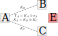
\includegraphics[draft=false, width=0.4\linewidth]{qss/qss_honest_recipients}
\caption{\label{fig:qss_honest_recipients} Alice will distribute her secret $\sigma_A$ to Bob and Charlie who are assumed honest. Dishonest Eve will try to attack the protocol and gain information about $\sigma_A$. Gray: honest. Red: dishonest. See Fig.~\ref{fig:qss_structure} for further information.}
\end{figure}


The starting point for our security analysis is the following Devetak-Winter bound \cite{Devetak2004} for the asymptotic key rate under collective attack, Fig.~\ref{fig:types_of_attack_collective},

%\MT{should I motivate why this bound is helpful for us?}

\begin{equation}\label{eqn:qss_dw_eve}
\kappa_{\text{Eve}} \ge \text{I}\left(X_A : X_B, X_C\right) - \chi\left(X_A : \mathbb{E}\right)
\end{equation}

\noindent which describes the balance between the mutual information, $\text{I}$, shared between Alice and a Bob-Charlie collaboration, and the Holevo information $\chi$ between Eve's quantum system $\mathbb{E}$ and Alice. It is perhaps unsurprising that Eq.~\ref{eqn:qss_dw_eve} should be our starting point given the noted similarities between QSS and QKD. The $X_A = \mathcal{F}\left(A_B, A_C\right)$ is Alice's variable based on her heterodyne measurement outcomes.

We would like to calculate the lower bound for key rate given by Eq.~\ref{eqn:qss_dw_eve} and so we will consider each term in turn and demonstrate how they may be calculated for the protocol described above.



\subsection{Mutual information}

Using Eq.~\ref{eqn:intro_mutual_information} the mutual information $\text{I}$ may be written as 
\begin{equation}\label{eqn:qss_deriv_1}
\text{I}\left(X_A : X_B, X_C\right) = \text{H}\left(X_B, X_C\right) - \text{H} \left(X_B, X_C \given X_A\right).
\end{equation}
where the first term on the right hand side is the joint Shannon entropy of $X_B$ and $X_C$, and the second term is the conditional Shannon entropy of $X_B, X_C$ given $X_A$, Sec.~\ref{sec:intro_shannon_entropy}. Intuitively this second term encodes the uncertainty one has about which $X_B, X_C$ were chosen, once Alice has formed $X_A$, while the first term encodes the \emph{a priori} entropy about Bob and Charlie's choice of sent coherent states.

The joint Shannon entropy may be written
\begin{equation}\label{eqn:qss_deriv_2}
\text{H}\left(X_B, X_C\right) = \sum_{X_B=b, X_C=c} - \text{P}\left(b, c\right) \log \text{P}\left(b, c\right)
\end{equation}
where $b, c$ are individual instances of variables $X_B, X_C$. In the following we shall take $b, c$ as phase elements of the QPSK alphabet, but this may be readily generalized to an $N$PSK alphabet. 

Since $b, c$ are taken to be independently chosen and uniformly random we see that the joint probability
\begin{equation}\label{eqn:qss_deriv_3}
\text{P}\left(b, c\right) = \text{P}\left(b\right)\times \text{P}\left(c\right) = \frac{1}{16}
\end{equation}
since each of the $b, c$ are chosen with probability $1/4$. We will relax this assumption in Chapter~\ref{chapter:aqc}.

Expanding the conditional entropy in $X_A$ via Eq.~\ref{eqn:intro_conditional_entropy_expansion} \cite{Wilde2013} we reach

\begin{equation}\label{eqn:qss_deriv_4}
\text{H}\left(X_B, X_C \given X_A\right) = \int\limits_{a \in \mathbb{C}} \Diff2 a \; \text{P}\left(X_A = a\right) \text{H}\left(X_B, X_C \given X_A = a\right),
\end{equation}
and we shall see that each term in Eq.~\ref{eqn:qss_deriv_4} can be calculated once function $\mathcal{F}$ is known. The conditional entropy $\text{H}\left(X_B, X_C \given X_A = a\right)$ expands as 

\begin{align}
\text{H}\left(X_B, X_C \given X_A=a\right) = - \sum_{b, c}  &\text{P}\left(X_B=b, X_C=c \given X_A=a\right) \times \notag \\
%
&\log \text{P}\left(X_B=b, X_C=c \given X_A=a\right) \label{eqn:qss_deriv_4_1}
\end{align}

\noindent and so all that remains is to calculate the probabilities 
\begin{align}
\label{eqn:qss_prob1} \text{P}\left(X_A=a\right) \qq{and} \\
\label{eqn:qss_prob2} \text{P}\left(X_B=b, X_C=c \given X_A=a\right)
\end{align}
with respect to a given function $\mathcal{F}$.


\subsubsection{Function $\mathcal{F}$}


We have no requirement that $\mathcal{F}$ should be injective. This implies, for example, that $\text{S}\left(\rho_{\left.\mathbb{E} \given A_B, A_C\right.}\right) \ne \text{S}\left(\rho_{\left. \mathbb{E} \given X_A\right.}\right)$, i.e. the entropy of Eve's quantum state conditioned on Alice's heterodyne outcomes $A_B, A_C$ is not equal to the entropy of Eve's quantum state conditioned on Alice's variable $X_A$, and so we must carefully consider the action of $\mathcal{F}$ early on in our analysis. 

To be concrete, in what follows we assume that $F$ is linear
\begin{equation}\label{eqn:qss_F_linear}
\mathcal{F}\left(x, y\right) := g x + h y \qq{with} g, h \in \mathbb{R}\setminus \left\{0\right\}
\end{equation} 
which will enable us to make some predictions about the performance of the protocol. Although we make no claims about the optimality of this choice of $\mathcal{F}$, we are free to optimize the key rate over $g, h$, and we will make it clear when we have done so. In Sec.~\ref{appendix:qss_moreF} we consider some alternative forms for $\mathcal{F}$.





\subsubsection{Expanding classical probabilities}

Applying Bayes' formula Eq.~\ref{eqn:intro_bayes} to probability Eq.~\ref{eqn:qss_prob2} we see that
\begin{align}
\text{P}\left(X_B=b, X_C=c \given X_A=a\right) = \text{P}&\left(X_A=a \given X_B=b, X_C=c\right) \notag \\
&\times \frac{\text{P}\left(X_B=b, X_C=c\right)}{\text{P}\left(X_A=a\right)}.
\end{align}


\noindent Now, we can access $\text{P}\left(X_A=a \given X_B=b, X_C=c\right)$. 
%by modelling the effects of the channel on quantum states distributed by Bob and Charlie. 
We take
\begin{equation}\label{eqn:qss_deriv_5}
X_A = \mathcal{F}\left(A_B, A_C\right) = g A_B + h A_C
\end{equation}
as in Eq.~\ref{eqn:qss_F_linear} and so we rearrange
\begin{equation}
A_C = \frac{X_A - g A_B}{h}.
\end{equation}

\noindent Since our $F$ is not injective %(there are multiple $A_B, A_C$ which will give the same $X_A$)
we must average over all of the possible ways to reach a given $X_A$. Therefore, once $X_A, g$ and $h$ are fixed, the choice of $A_B, A_C$ reduces to a one-variable problem. So

\begin{equation}\label{eqn:qss_deriv_5_1}
\text{P}\left(X_A \given X_B=b, X_C=c\right) = \int\limits_{A_B \in \mathbb{C}} \Diff2 A_B \; \text{P}\left(A_B , \frac{X_A - g A_B}{h} \given X_B=b, X_C=c\right)
\end{equation}
which may be calculated once we know how the channel acts on input states. Note that an analogous expression would be reached by rearranging Eq.~\ref{eqn:qss_deriv_5} as $A_B = \left(X_A - h A_C\right)/g$, but it will make no difference to the resulting quantities which we derive from Eq.~\ref{eqn:qss_deriv_5_1}

Assuming that the two channels, one from Charlie$\rightarrow$Alice and one from Bob$\rightarrow$Alice, are independent from each other\footnote{We shall see later what this means for their combined action on an input quantum state} allows us to write
\begin{equation}\label{eqn:qss_deriv_6}
\text{P}\left(A_B, A_C \given X_b=b, X_C=c\right) = \text{P}\left(A_B \given X_B=b\right) \times \text{P}\left(A_C \given X_C=c\right)
\end{equation}
for the probabilities that Alice's heterodyne measurement outcomes are $A_B, A_C$ if coherent states with phases $\phi_B = b, \phi_C = c$ are sent.

Let us assume for now that each channel is noiseless but lossy. The probability that Alice measures a particular heterodyne outcome $a \in \mathbb{C}$ when a coherent state of complex amplitude $\beta$ is sent through a lossy channel, transmittivity $T$, is (Sec.~\ref{sec:qss_perr}) %where do I actually derive this? I should put it in one place and then refer to it a bunch
\begin{equation}\label{eqn:qss_channel_classical_prob}
\text{P}\left(a \given \beta, T\right) = \frac{1}{\pi}\exp\left( - \left| a - \sqrt{T}\beta \right|^2\right)
\end{equation}
which we have used previously in Ch.~\ref{chapter:qds}. The required changes to include thermal noise of the channel can be readily made, Sec.~\ref{sec:thermal_channel}.

The integral in Eq.~\ref{eqn:qss_deriv_5_1} may be calculated analytically to reach 
\begin{align}\label{eqn:qss_deriv_7}
\text{P}\left(X_A \given X_B=b, X_C=c\right) = \frac{1}{\pi} \frac{1}{g^2 + h^2} &\exp \left( - \frac{\left[b^R g \sqrt{T_B} + c^R h \sqrt{T_C} - X_A^R \right]^2}{g^2 + h^2}\right) \notag \\
%
&\times \exp \left( - \frac{\left[b^I g \sqrt{T_B} + c^I h \sqrt{T_C} - X_A^I \right]^2}{g^2 + h^2} \right)
\end{align}
where $b, c$ are Bob and Charlie's coherent state amplitudes, $X_A$ is Alice's final variable after applying $\mathcal{F}$ Eq.~\ref{eqn:qss_F_linear} to her heterodyne outcomes, $T_B, T_C$ are the transmittivities of the Bob$\rightarrow$Alice channel and Charlie$\rightarrow$Alice channel, respectively, and a superscript $R\left(I\right)$ denotes the real (imaginary) part of the corresponding quantity. %\MT{I probably don't need to say much about how this integration is actually done, since it should be obvious.} 
The probability $\text{P}\left(X_A=a\right)$ Eq.~\ref{eqn:qss_prob1} may now be found by %summing Eq.~\ref{eqn:qss_deriv_7} over all $b, c$ in our QPSK alphabet.

\begin{equation}\label{eqn:qss_deriv_pxa}
\text{P}\left(X_A\right) = \sum_{b, c} \text{P}\left(X_A \given X_B=b, X_C=c\right).
\end{equation}






Finally, the mutual information Eq.~\ref{eqn:qss_deriv_1} may be calculated. We perform the integration over $X_A$ in Eq.~\ref{eqn:qss_deriv_4} numerically and display the mutual information $I$ in Fig.~\ref{fig:qss_mutinf_graphs}.


% Have some graphs of the various probabilities and mutual information


%Let us now explore how the mutual information behaves. \MT{Now let's make some graphs and really have fun exploring how $I$ behaves.}

\subsection{Holevo information}

We will now detail how the Holevo information term in Eq.~\ref{eqn:qss_dw_eve} may be calculated. In doing so we will point to areas where future work might strengthen the security analysis to consider wider classes of attack, which should illuminate the contexts to which our security proof may be applied. In this section we consider a dishonest Eve performing attack BS$0$, as detailed above in Sec.~\ref{sec:qds_bs0}, though the analysis follows readily for the other attacks described in Sec.~\ref{sec:qds_attack_analysis}. We will then compare the strength of attacks BS$0$, BS$1$, BS$2$ and EC. % and more general attacks will be considered later.

Bob and Charlie prepare a state from the QPSK alphabet, and each state is chosen randomly and with equal probability. Before the channel, Bob and Charlie hold the joint state
\begin{equation}
\rho_{\text{before}} = \rho_B \otimes \rho_C
\end{equation}
with
\begin{equation}
\rho_B = \frac{1}{4} \sum_{k=0}^3 \dyad{\beta_k}_B \qq{and} \rho_C = \frac{1}{4} \sum_{k^\prime = 0}^3 \dyad{\gamma_{k^\prime}}_C
\end{equation}
where $\beta, \gamma$ are the amplitudes of Bob's and Charlie's coherent state alphabets.\footnote{These complex amplitudes $\beta, \gamma$ were denoted $b, c$ in the previous section.}

We assume that the channel acts separately on each mode, and that modes $\rho_B$, $\rho_C$ undergo independent evolution. In other words, we assume that the channel has the following structure
\begin{equation}\label{eqn:qss_channel}
\Phi\left[\rho\right] = \Phi_B\left[\rho\right] \otimes \Phi_C\left[\rho\right]
\end{equation}
where $\Phi_{B, C}$ denote the lossy channels described by attack BS$0$, Sec.~\ref{sec:qds_bs0}, and the subscript $B, C$ denotes which mode of $\rho_{\text{before}}$ each channel acts on. 
\iffalse
\begin{align}
\Phi_B\left[\rho\right] = \varphi_B\left(\text{Tr}_C \rho\right) \otimes \mathds{1}_C\left(\text{Tr}_B\rho\right) \notag \\
\Phi_C\left[\rho\right] = \mathds{1}_B\left(\text{Tr}_C\rho\right) \otimes \varphi_C\left(\text{Tr}_B\rho\right)
\end{align}
with $\mathds{1}$ the identity channel and $\varphi_{B,C}$ denotes the lossy channels described by attack BS$0$, Sec.~\ref{sec:qds_bs0}. The Total 
\fi
The total channel $\Phi$ preserves the tensor-product structure of the input state.

Physically $\Phi$ corresponds to the case where Eve performs separate beamsplitter attacks on each channel and retains two output modes $\mathbb{E}_{B, C}$, Fig.~\ref{fig:qss_bs0_attack}.

\begin{figure}[htp]
\centering
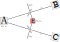
\includegraphics[draft=false, width=0.8\linewidth]{qss/qss_bs0}
\caption{\label{fig:qss_bs0_attack} We model the channel $\Phi$ as two independent beamsplitter attacks of type BS$0$, Sec.~\ref{sec:qds_bs0}. This preserves the tensor-product structure of $\rho_{\text{before}}$.}
\end{figure}


The total state after the channel becomes
\begin{equation}
\rho_{\text{after}} = \rho_{\mathbb{A}_B, \mathbb{E}_B} \otimes \rho_{\mathbb{A}_C, \mathbb{E}_C}
\end{equation}
with $\mathbb{A}_{B, C}$ denoting Alice's two modes and where
\begin{equation}
\rho_{\mathbb{A}_B, \mathbb{E}_B} = \frac{1}{4} \sum_{k=0}^3 \dyad{\sqrt{T_B} \beta_k}_{\mathbb{A}_B} \otimes \dyad{\sqrt{1-T_B} \beta_k}_{\mathbb{E}_B}
\end{equation}
and similarly for $\rho_{\mathbb{A}_C, \mathbb{E}_C}$. Now, Alice heterodynes and measures $A_B \in \mathbb{C}$ from $\rho_{\mathbb{A}_B, \mathbb{E}_B}$ and $A_C \in \mathbb{C}$ from $\rho_{\mathbb{A}_C, \mathbb{E}_C}$. Eve's total state conditioned on these outcomes becomes 
\begin{equation}\label{eqn:qss_eve_conditional}
\rho_{\left.\mathbb{E} \given A_B, A_C\right.} = \rho_{\left.\mathbb{E}_B \given A_B\right.} \otimes \rho_{\left. \mathbb{E}_C \given A_C\right.}
\end{equation}
with
\begin{equation}
\rho_{\left.\mathbb{E}_B \given A_B\right.} = \frac{1}{4 \pi} \sum_{k=0}^3 \text{P}_B\left(A_B \given \beta_k, T_B\right) \dyad{\sqrt{1-T_B} \beta_k}_{\mathbb{E}_B}
\end{equation}
and similarly for $\rho_{\left.\mathbb{E}_C \given A_C\right.}$. The probability $\text{P}_B\left(A_B \given \beta_k, T_B\right)$ is calculated analogously to Eq.~\ref{eqn:qss_channel_classical_prob}, and similarly for $A_C$.

To proceed, we take $X_A = g A_B + h A_C$ as usual, with $g, h$ fixed, and write $A_C = \left(X_A - g A_B\right)/h$. Therefore the state $\rho_{\left.\mathbb{E} \given A_B, A_C\right.}$, Eq.~\ref{eqn:qss_eve_conditional}, becomes

\begin{align}\label{eqn:qss_deriv_8}
\rho_{\left. \mathbb{E} \given X_A, A_B\right.} &= \frac{1}{16 \pi^2} \sum_{k, k^\prime = 0}^3 \text{P}_B\left(A_B \given \beta_k, T_B\right) \text{P}_C\left(\frac{X_A - g A_B}{h} \given \gamma_{k^\prime}, T_C\right) \notag \\
%
&\dyad{\sqrt{1-T_B} \beta_k}_{\mathbb{E}_B} \otimes \dyad{\sqrt{1-T_C}\gamma_{k^\prime}}_{\mathbb{E}_C}
\end{align}

\noindent Once again since Alice's function $\mathcal{F}$ is in general not injective we must mix over outcomes $A_B, A_C$ in order to find Eve's state $\rho_{\left.\mathbb{E} \given X_A\right.}$. Therefore 

\begin{equation}\label{eqn:qss_aposteriori_state}
\rho_{\left.\mathbb{E} \given X_A\right.} = \int\limits_{A_B \in \mathbb{C}} \Diff2 A_B \; \text{P}\left(A_B\right) \rho_{\left.\mathbb{E} \given X_A, A_B\right.}
\end{equation}

\noindent and mixing over $X_A$ we finally reach

\begin{equation}\label{eqn:qss_apriori_state}
\rho_{\mathbb{E}} = \int\limits_{X_A \in \mathbb{C}} \Diff2 X_A \; \text{P}\left(X_A\right) \rho_{\left.\mathbb{E}\given X_A\right.}.
\end{equation}

\noindent We may identity Eq.~\ref{eqn:qss_aposteriori_state} as Eve's \emph{a prosteriori} state and Eq.~\ref{eqn:qss_apriori_state} as Eve's \emph{a priori} state and so Eve's Holevo information is given by the usual formula

\begin{equation}\label{eqn:qss_holevo}
\chi = \text{S}\left(\rho_\mathbb{E}\right) - \int\limits_{X_A \in \mathbb{C}} \Diff2 X_A \; \text{P}\left(X_A\right) \text{S}\left(\rho_{\left.\mathbb{E} \given X_A\right.}\right).
\end{equation}
where we note that we can no longer simplify the second term in Eq.~\ref{eqn:qss_holevo}, as we did in Sec.~\ref{sec:qds_attack_analysis}, for example, since in general each state $\rho_{\left.\mathbb{E} \given X_A\right.}$ will have a different entropy.


\noindent Let us explore the behaviour of Eve's Holevo information Eq.~\ref{eqn:qss_holevo}.

\MT{TODO: make some nice graphs of $\chi$ in different scenarios and under different attacks BS1, BS2, EC.}

\section{Security against a dishonest player}
%\MT{Talk about guarding against a dishonest Bob/Charlie.}
Of course, if Alice only had to guard against an external Eve, and both Bob and Charlie could be assumed honest, then the QSS task becomes much easier. She could, for example, simply send the same information to each recipient. Or send her secret just to the recipient she is interested in, with no need to ``split'' it or share it. 

\subsection{Dishonest Bob}
Let us translate the analysis from Sec.~\ref{sec:qss_honest_recipients} to the case where either Bob or Charlie is dishonest, but Alice does not know which one, Fig.~\ref{fig:qss_structure}. Including a dishonest recipient in the above security proof requires us to re-calculate several quantities. For concreteness we will first assume that Bob is dishonest and Charlie is honest, Fig.~\ref{fig:qss_dishonest_Bob}, and we will allow Bob to collaborate with Eve. Later we will discuss how to account for the fact that we do not know \emph{which} player is dishonest.

\begin{figure}[htp]
\centering
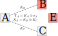
\includegraphics[draft=false, width=0.6\linewidth]{qss/qss_dishonest_Bob}
\caption{\label{fig:qss_dishonest_Bob} A dishonest Bob gains an advantage since he knows which coherent state he chose to send to Alice. He may additionally choose to collaborate with Eve in order to gain information about Alice's measurement on Charlie's state. c.f. Fig.~\ref{fig:qss_structure}.}
\end{figure}

The main effect of permitting dishonesty from Bob is that he knows precisely which coherent states he sent to Alice. This will give him reduced uncertainty about Alice's variable $X_A$. Bob might also wait and see which coherent state was sent by Charlie before choosing his own, in order to preference a certain outcome $X_A$. \MT{Make some comments about this.} We will assume that Bob sends states only from the QPSK alphabet, though in principle this could be relaxed in future work.

Since Bob knows which coherent states he sent we must re-calculate several expressions from Sec.~\ref{sec:qss_honest_recipients} with the key change that we no longer mix over Bob's alphabet. The quantities which this influences are

\begin{equation}
\text{P}\left(X_A=a\right) = \sum_{c} \text{P}\left(X_A \given X_b=b, X_C=c\right)
\end{equation}

\noindent and

\begin{align}
\text{H}\left(X_B, X_C \given X_A=a\right) = - \sum_{c} \text{P}&\left(X_B=b, X_C=c \given X_A=a\right) \times \notag \\
&\log \text{P}\left(X_B=b, X_C=c \given X_A=a\right)
\end{align}

\noindent and the mutual information may now be calculated as in the previous section. 

The Holevo information is also calculated analogously to the previous section, the key change being that Eve's state conditioned on $X_A, A_B$, Eq.~\ref{eqn:qss_deriv_8}, is now given by
\begin{align}\label{eqn:qss_deriv_9}
\rho_{\left.\mathbb{E} \given X_A, A_B\right.} &= \frac{1}{4 \pi^2} \sum_{k^\prime=0}^3 \text{P}_B\left(A_B \given \beta_k, T_B\right) \text{P}_C\left(\frac{X_A - g A_B}{h} \given \gamma_{k^\prime}, T_C\right) \notag \\
%
&\dyad{\sqrt{1-T_B} \beta_k}_{\mathbb{E}_B} \otimes \dyad{\sqrt{1-T_C}\gamma_{k^\prime}}_{\mathbb{E}_C}
\end{align}
and the \emph{a posteriori} and \emph{a priori} states calculated by integrating Eq.~\ref{eqn:qss_deriv_9} identically to Eqs.~\ref{eqn:qss_aposteriori_state},~\ref{eqn:qss_apriori_state}.

Since we no longer mix over Bob's coherent state $b$, the mutual information $\text{I}$ and Holevo information $\chi$ have become functions of $b$. In this chapter we assume that each state in the QPSK alphabet is equally likely and has equal magnitude and so both $\text{I}$ and $\chi$ will be identical for each of Bob's alphabet states. We will relax this in Chapter~\ref{chapter:aqc}.


The final key rate is now
\begin{equation}\label{eqn:qss_keyrate_dishonest_Bob}
\kappa_{\text{Eve, Bob}} = \text{I}\left(X_A : X_B, X_C\right) - \chi\left(X_A : \mathbb{E} \mathbb{B}\right)
\end{equation}
with mutual information and Holevo information terms calculated as described above.


%\MT{Make some graphs of things with dishonest Bob}


\subsection{Dishonest Bob or Dishonest Charlie}
If Alice is certain that Bob is the dishonest player then she has no need for a secret sharing scheme. Equivalently, she can set $g=0$ in her function $\mathcal{F}$. If she is correct about Bob's dishonestly, then she has successfully prevented him from gaining any information about her secret. However, if Alice turns out to be wrong and it is Charlie who is the dishonest player then she has accidentally given Charlie the secret! It is the uncertainty about which player is dishonest which makes a QSS scheme necessary.

In order to take into account this uncertainty over which player is dishonest, Fig.~\ref{fig:qss_structure}, we proceed as in the recent QSS works Refs.~\cite{Kogias2017, Grice2019} and calculate the minimum over all possible dishonest configurations. That is, we take

\begin{equation}
\kappa \ge \min \left\{\kappa_{\text{Eve, Bob}}, \kappa_{\text{Eve, Charlie}}\right\}
\end{equation}
where $\kappa_{\text{Eve, Charlie}}$ is calculated analogously to Eq.~\ref{eqn:qss_keyrate_dishonest_Bob}. \MT{Comment about why this works.}


\section{Protocol performance}
\MT{Make some graphs of key rate and tweak all of the parameters that I can in all of the attacks that I can.}

\MT{If I have time, make some graphs with e.g. homodyning instead of heterodyning, or different alphabets.}

















\section{Outlook}
%\MT{this section should be somewhere else, perhaps in an "outlook" section?}
The classical post-processing of the above protocol is inherently very similar to Ref.~\cite{Kogias2017}, in which a secret key is generated between Alice and a shared Bob-Charlie degree of freedom via incompatible homodyne measurements on a tripartite entangled state. We expect that our protocol will be secure against a more restricted set of attacks, but over a wider range of channel parameters, for several reasons. 

Firstly unlike Ref.~\cite{Kogias2017} which relies in generation and distribution of large multipartite entangled states, our scheme has much more modest quantum requirements which are known to be easy to generate and manipulate, and which will be much more robust to channel loss and channel noise than a large entangled state. Quantum cryptography using continuous-variables typically operates over metropolitan distances of tens of kilometers, and so we might reasonably expect similar performance of our QSS protocol. Performance of our protocol over a realistic fiber channel is analysed in Chapter~\ref{chapter:aqc}. 

Secondly, the protocol from Ref.~\cite{Kogias2017} takes a form analogous to direct-reconciliation (DR) QKD, while ours is analogous to reverse-reconciliation (RR) QKD. RR QKD is known \cite{Grosshans2002, Grosshans2003, Laudenbach2017} to be much more resilient to loss and noise than DR QKD without modifications \cite{Silberhorn2002}.

Ref.~\cite{Kogias2017} has potentially dishonest players Bob and Charlie performing homodyne measurements on incompatible observables (i.e. switching between $q$ and $p$ quadratures). No assumptions are made about the measurement devices used and they are each treated as a "black-box". Security comes inherently because of a Heisenberg-type relation between incompatible observables, and the security proof relies on an Entropic Uncertainty Relation (EUR) whic hhave had success in many parts of quantum cryptography \cite{Furrer2012, Furrer2017}. However, since we desire to use heterodyne detection we are forced to adopt a different approach and explicitly model the states' evolution and measurement during the protocol. We note that this matches the current state-of-the-art of QPSK-based QKD \cite{Papanastasiou2018}, but should be improved in future work.

We have assumed that a dishonest Bob or Charlie still sends a state from the QPSK alphabet. It is yet unclear whether they could gain an advantage by sending something exotic and potentially highly entangled, perhaps in order to force Alice to reach a certain key $X_A$. This should be explored and potentially relaxed in future work. We anticipate that applying methods from quantum bit commitment \cite{Broadbent2015} might prove fruitful here, since bit commitment also relies on a potentially dishonest distribution of the quantum state.

Finally, we note that our assumption that the channel between Alice and Bob-Charlie takes a tensor-product structure, Eq.~\ref{eqn:qss_channel}, Fig.~\ref{fig:qss_bs0_attack} is a strong one and should be relaxed. A potential strategy of a dishonest player could be to exploit properties of a general channel which maps a two-mode input state to a two-mode output state at Alice, potentially allowing a dishonest player many output ancilla modes correlated with Alice. Such a strategy will be restricted by the conditions that the reduced state of an honest player should be a coherent state (with noise). Similarly it will require that Alice's measurement outcomes don't look ``too errant'', though this should be quantified.









%\chapter{Agile quantum cryptography}
Goal of chapter: introduce and make explicit the concept of quantum agility in quantum cryptography. Join together several threads from the previous two chapters. This chapter can be viewed as a "bonus" to the QDS and QSS chapters.

\iffalse
Key things I want to present, in roughly the order that I want to present them:

\begin{itemize}
\item Discussion of agility and why it might be desirable. Motivate it in terms of my two literature reviews.
\item Modification of QDS protocol from earlier to be agile with QSS (i.e. introduce protocol QSS-b and prove its security (inc postselection)). Have some graphs of its behaviour
\item Bring in QKD from the literature (Papanastasiou2018). Have some graphs of its behaviour and discussion of how it relates to my thesis.
\item Talk about the experiment (emphasise that it is not my work). I can have some plots of raw data (opendata), and make graphs of data points which I received.
\item Analysis of the data under each protocol with discussion of how results from previous chapters are modified to make them more realistic
\item Graphs of performance at different data parameters
\item Table from the AQC paper $\leftarrow$ this can be the climax of this section
\item star graph of QDS
\item Discussion of how our analysis motivates agility
\item Outlook/next steps
\end{itemize}
\fi

\section{Introduction}

% Review some things from my previous two literature reviews
We have observed over the past two chapters, and in our overviews of quantum cryptography in Chapter~\MT{X}, that several quantum cryptographic protocols are intimately related. As Simmons noted

\MT{insert simmons quote}

and so we have seen close connections between QKD and QSS, and QSS may be interpreted simply as QKD performed between one player (dealer) and several players (recipients of the secret). We have also remarked that the secret sharing task may be performed pseudo-classically, by first encrypting channels using QKD and then using an unconditionally secure classical secret sharing protocol. 

It was noted \MT{cite some papers} that QSS is related to quantum conferencing and often the same hardware setup may be used to perform both tasks. And in Ref.~\MT{cite} it was explicitly demonstrated that a round-robin QSS protocol can also be used to perform QKD between any two players. Moving to the QDS literature, ever since discovery of practical QDS requiring neither quantum memory, entanglement or an optical multiport that there are close links between QDS and QKD. Ref.~\MT{cite} explicitly builds their QDS protocol to use QKD hardware, while Ref.~\MT{cite} realise a setup which can, with minimal hardware modification, perform either QDS or QKD, with additional MDI capabilities. And in Refs.~\MT{cite a bunch of stuff} it was explicitly remarked that QDS differs from QKD \emph{only} in the classical postprocessing. Finally, in Ref.~\MT{cite} the authors design their QSS scheme on the same principles as DPS QKD \MT{define and check}. And many papers build their security proofs on techniques designed for QKD \MT{cite loads of stuff.}

%We therefore might ask 

It should be clear that the field of quantum cryptography is far broader than mere QKD. As we move closer towards practical implementation of diverse quantum cryptographic protocols we must consider not only the unconditional security of the underlying protocol, but also its ease of implementation. As protocols are designed with minimal and often overlapping hardware requirements we may ask the question:
\\
\par
\emph{given a particular hardware setup, which quantum protocols can I perform?}
\\
\\
\noindent Or, desiring a large-scale quantum cryptographic network:
\\
\par
\emph{given a deployed network architecture, which quantum protocols can I perform with minimal disruption?}
\\
\\
\noindent Both of these questions have deep impacts on the success probability of a future large-scale quantum network. \MT{Chat more about the networks. Mention DV over installed fibers results from recent years. (Did they require dedicated hardware?)}

We have already even seen several quantum routes to accomplishment of the same task. By first utilizing QKD between all players it is possible to perform DS \MT{cite} or SS \MT{cite} using unconditionally secure classical algorithms, and indeed this may often be preferable to protocols requiring large entangled states \MT{cite}. Alternatively, in a distributed quantum computing setup which can easily generate and distribute entanglement, a protocol such as Ref.~\MT{cite} may be advantageous if it takes advantage of already accessible hardware. 





%\part{PhoG: generation of sub-Poissonian light}
%%
% A (non-exhaustive) list of TODOs:
%
% - write appendix displaying adiabatic elimination of a lossy mode for an arbitrary operator. 

\chapter{PhoG: Photon Gun}\label{chapter:phog}
Goal of chapter: analyse and model the PhoG device and its efficacy for producing, from a classical input, (i) bright sub-Poissonian state; (ii) entangled state


\section{Introduction}
\begin{itemize}
\item Introduce dissipation as a means for state engineering
\item Introduce our goal to produce single-photons (or close to single-photons)
\item Introduce this chapter, include a chapter outline, and provide motivation for why we will look at different models
\end{itemize}

\begin{figure}[htp]
\centering
\includegraphics[draft=false, width=\linewidth]{phog/phog_models}
\caption{\label{fig:phog_models} Hierarchy of models of the phog device, from least realistic (left) to most realistic (right). We will discuss each model in turn throughout the rest of this chapter. \MakeUppercase{\romannumeral 1}: Single-mode model. \MakeUppercase{\romannumeral 2}: Two-mode model. \MakeUppercase{\romannumeral 3}: Three-mode model. \MakeUppercase{\romannumeral 4}: Multi-mode model. \MakeUppercase{\romannumeral 5} Multi-mode model embedded in glass. }
\end{figure}

\section{Single-mode model}\label{sec:phog_single_mode_model}

\begin{figure}[htp]
\centering
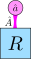
\includegraphics[width=0.2\linewidth, draft=false]{phog/single_mode}
\caption{\label{fig:phog_single_mode} A single bosonic mode, $a$, is coupled to a Markovian reservoir $R$ by operator $\hat{A}$. }
\end{figure}

\MT{Make sure that my analysis in this section is sufficiently motivated and doesn't seem like too much of a detour.}

Consider the model displayed in Fig.~\ref{fig:phog_single_mode} (c.f. Fig.~\ref{fig:phog_models}\MakeUppercase{\romannumeral 1}), which consists of a single bosonic mode, $a$, coupled to a reservoir $R$ via a reservoir operator $\mathcal{A}$. The annihilation (creation) operator for mode $a$ is denoted $\hat{a} \left(\hat{a}^\dagger\right)$, and the density matrix containing all information about the state of the mode is denoted $\rho_a$. This model will prove illustrative of several principles which we will develop throughout the chapter. Assuming that reservoir $R$ is Markovian, the evolution of mode $a$ is given by the following quantum master equation in Lindblad form\footnote{Equations in this form will be referred to as ``Lindblad equations''}

\begin{equation}\label{eqn:phog_lindblad_1}
\ddt \rho_a =  - i \left[\hat{H}, \rho_a\right] + \gamma \mathcal{L}\left(\hat{A}\right)\rho_a
\end{equation}

\noindent In what follows we consider the case with Hamiltonian $\hat{H} = \hbar \omega \hat{a}^\dagger \hat{a}$. Eq.~\ref{eqn:phog_lindblad_1} then describes the decay of state $\rho_a\left(t=0\right)$ into $R$ with rate $\gamma$. The Lindbladian term $\mathcal{L}\left(\hat{A}\right)$ takes the usual form
\begin{equation}\label{eqn:phog_lindbladian_form}
\mathcal{L}\left(\hat{A}\right)\rho_a = \hat{A}\rho_a\hat{A}^\dagger - \frac{1}{2} \hat{A}^\dagger \hat{A} \rho_a - \frac{1}{2} \rho_a \hat{A}^\dagger \hat{A}.
\end{equation}

\noindent Let us consider the behaviour of an initially coherent state $\rho_a\left(t=0\right) = \dyad{\alpha}$ with amplitude $\alpha$. We will explore several choices for decay operator $\hat{A}$.

\subsection{$\hat{A} = \hat{a}$}
First, we will explore the case where the decay into the reservoir is governed by mode $a$ annihilation operator, $\hat{a}$, which corresponds to single-photon loss.% I can refer to intro chapter for properties of this.
The evolution of $\rho_a$ is described by

\begin{equation}\label{eqn:phog_lindblad_single_photon_loss}
\ddt \rho_a = \gamma\left[\hat{a}\rho_a \hat{a}^\dagger - \frac{1}{2} \hat{a}^\dagger \hat{a} \rho_a - \frac{1}{2} \rho_a \hat{a}^\dagger \hat{a}\right],
\end{equation}
where we have transformed into a rotating frame and so the free Hamiltonian term $\hbar \omega \hat{a}^\dagger \hat{a}$ vanishes. Let us calculate the evolution $\langle \hat{a}^\dagger \hat{a}\rangle\left(t\right)$ of photon number expectation:

\begin{align}
\ddt \langle \hat{a}^\dagger \hat{a}\rangle &= \gamma \left[ \text{Tr}\left(\hat{a}^\dagger \hat{a} \hat{a} \rho_a \hat{a}^\dagger \right) - \frac{1}{2} \text{Tr}\left(\hat{a}^\dagger \hat{a} \hat{a}^\dagger \hat{a} \rho_a\right) - \frac{1}{2} \text{Tr}\left(\hat{a}^\dagger \hat{a} \rho_a \hat{a}^\dagger \hat{a}\right)\right] \notag \\
%
&= \gamma \left[ \langle \hat{a}^\dagger \hat{a}^\dagger \hat{a}\hat{a}\rangle - \langle \hat{a}^\dagger \hat{a} \hat{a}^\dagger \hat{a}\rangle \right] \notag \\
%
&= - \gamma \langle \hat{a}^\dagger \hat{a}\rangle
\end{align}
\noindent and so
\begin{equation}\label{eqn:phog_single_photon_loss_number_expectation}
\langle\hat{a}^\dagger \hat{a} \rangle \left(t\right) = \langle \hat{a}^\dagger \hat{a}\rangle \left(0\right) e^{- \gamma t}
\end{equation}
the photon number exponentially decays in time with decay rate $\gamma$. We may derive similar equations for $\langle\hat{x}\rangle\left(t\right)$ and $\langle\hat{x}\rangle\left(t\right)$ and find 
\begin{align}\label{eqn:phog_single_photon_loss_quadrature_expectation}
 \langle \hat{x}\rangle\left(t\right) &= \langle \hat{x}\rangle\left(0\right) e^{- \frac{\gamma}{2} t} \notag \\
%
 \langle \hat{p}\rangle\left(t\right) &= \langle \hat{p}\rangle \left(0\right) e^{- \frac{\gamma}{2} t}.
\end{align}

\noindent We might guess that the steady-state of Eq.~\ref{eqn:phog_lindblad_single_photon_loss} is the vacuum $\dyad{0}$, and indeed we can deduce that this must be the case by noticing that $\ddt \rho_a = 0$ when $\rho_a$ is vacuum. In Fig.~\ref{fig:phog_lindblad_single_photon_loss}a we plot the evolution of $\langle\hat{a}^\dagger \hat{a}\rangle, \langle \hat{x}\rangle, \langle \hat{p}\rangle$ and see that the photon number expectation and quadrature expectations decay towards zero, confirming Eqs.~\ref{eqn:phog_single_photon_loss_number_expectation},~\ref{eqn:phog_single_photon_loss_quadrature_expectation}, while the variances in $\hat{x}$ and $\hat{p}$ remain constant. This might lead us to conclude that the state $\rho_a\left(t\right)$ remains a coherent state with decreasing amplitude $\alpha\rightarrow0$, until it reaches the vacuum state.

In Fig.~\ref{fig:phog_lindblad_single_photon_loss}b we plot the fidelities $\mathcal{F}$ between $\rho_a\left(t\right)$ and the vacuum state $\dyad{0}$, the single-photon state $\dyad{1}$ and a coherent state $\dyad{\alpha^\prime}$ with $\left|\alpha^\prime\right|^2 = \langle \hat{n}\rangle_{\rho_a}\left(t\right)$, in other words the coherent state with same photon-number expectation as $\rho_a$. We observe that the fidelity to the vacuum state increases to $1$ while the fidelity to coherent state $\dyad{\alpha^\prime}=1$ always, which confirms our intuitions that $\rho_a$ remains coherent $\forall t$ and that $\dyad{0}$ is the steady state.


\begin{figure}[htp]
\centering
	\begin{subfigure}{0.6\linewidth}
	\centering
	\includegraphics[draft=false, width=\linewidth]{phog/expects_a}
	\caption{}
	\end{subfigure}
	\begin{subfigure}{0.6\linewidth}
	\centering
	\includegraphics[draft=false, width=\linewidth]{phog/fidelities_a}
	\caption{}
	\end{subfigure}
\caption{\label{fig:phog_lindblad_single_photon_loss}$\hat{A} = \hat{a}$. (a) Operator expectation values calculated for state $\rho_a\left(t\right)$ as it evolves under Eq.~\ref{eqn:phog_lindblad_single_photon_loss}. An initial coherent state $\alpha=3.0$ decays to vacuum state $\dyad{0}$. Quadrature variances remain constant through time, implying that $\rho_a$ remains a coherent state throughout its evolution. This is confirmed in (b) where the fidelity between $\rho_a$ and $\dyad{\alpha^\prime}$ is demonstrated to remain $1$ for all time. The amplitude $\alpha^\prime$ is chosen to give a coherent state with equivalent photon-number expectation to $\rho_a\left(t\right)$. Horizontal gridlines displayed in black, dashed.}
\end{figure}

\subsection{$\hat{A} = \hat{a}^2$}
Next we consider a two-photon loss term $\hat{a}^2$, which describes two-photon decay into the reservoir. Our Lindblad equation is

\begin{equation}\label{eqn:phog_lindblad_two_photon_loss}
\ddt \rho_a = \gamma\left[\hat{a}^2 \rho_a \hat{a}^{\dagger 2} - \frac{1}{2} \hat{a}^{\dagger 2} \hat{a}^2 \rho_a - \frac{1}{2} \rho \hat{a}^{\dagger 2} \hat{a}^2\right]
\end{equation}
which gives the evolution of photon number expectation as 
\begin{equation}
\ddt \langle \hat{a}^\dagger \hat{a}\rangle = - 2 \gamma \langle \hat{a}^\dagger \hat{a}^\dagger \hat{a}\hat{a}\rangle
\end{equation}
which does not take a closed form and so we cannot yet directly calculate $\langle \hat{a}^\dagger \hat{a}\rangle\left(t\right)$. Similarly, equations for evolution of $\langle\hat{a}\rangle\left(t\right)$ require terms to the third power in the creation/annihilation operators, and so are not yet closed.  We will see techniques in Sec.~\ref{sec:linearization} which allow us to deal with this.

\MT{TODO: expand this discussion to allow for mixedness in output state.}
For now, let us deduce what must be the steady-state of Eq.~\ref{eqn:phog_lindblad_two_photon_loss}. We observe that once again the vacuum $\dyad{0}$ must be a steady state, since then $\ddt \rho_a=0$. Surprisingly we now also have the single-photon state $\dyad{1}$ as a steady state since this also has $\ddt \rho_a=0$. The general steady-state is a superposition of these
\begin{equation}\label{eqn:phog_phase_state}
\ket{\psi} = \ket{0} + e^{i \phi} \ket{1} \qq{with} \rho_a\left(t \rightarrow \infty\right) = \dyad{\psi}
\end{equation}
which takes the form of a so-called \emph{phase state}, and has long been known that the steady state of two-photon loss is a phase-state. The phase $\phi$ is related to the phase of the initial coherent state. %\MT{show this.}


In Fig.~\ref{fig:phog_lindblad_two_photon_loss}a we plot the evolution of $\langle \hat{a}^\dagger \hat{a}\rangle, \langle \hat{x}\rangle, \langle \hat{p}\rangle$ and the quadrature variances. The photon number expectation no longer decays to zero as it did for $\hat{A}=\hat{a}$. In Fig.~\ref{fig:phog_lindblad_two_photon_loss}b we observe the fidelity between $\rho_a\left(t\right)$ and the final phase state increases to $\MT{X}$, and so we see that two-photon loss induces nonclassicality in the system. \MT{I should talk about the mixedness of the state somewhere.}


\begin{figure}[htp]
\centering
	\begin{subfigure}{0.6\linewidth}
	\centering
	\includegraphics[draft=false, width=\linewidth]{phog/expects_aa}
	\caption{}
	\end{subfigure}
	\begin{subfigure}{0.6\linewidth}
	\centering
	\includegraphics[draft=false, width=\linewidth]{phog/fidelities_aa}
	\caption{}
	\end{subfigure}
\caption{\label{fig:phog_lindblad_two_photon_loss}$\hat{A} = \hat{a}^2$. (a) Operator expectation values for state $\rho_a\left(t\right)$ as it evolves under Eq.~\ref{eqn:phog_lindblad_two_photon_loss}. An intially coherent state with $\alpha=3.0$ no longer decays to the vacuum state, and the final photon-number expectation is nonzero. The quadrature variances are no longer constant which implies that the state is no longer coherent, which is confirmed in (b) where the fidelity between $\rho_a\left(t\right)$ and $\dyad{\alpha^\prime}$ is plotted. The fidelity between $\rho_a\left(t\right)$ and steady state increases to \MT{X}. Horizontal gridlines displayed in black, dashed.}
\end{figure}



\subsection{$\hat{A} = \hat{a}^3$}
We might guess that the steady state $\ket{\psi}$ of the three-photon loss term $\hat{a}^3$ is likewise a superposition of $\ket{0}, \ket{1}$ and $\ket{2}$
\begin{equation}\label{eqn:phog_three_photon_loss_ss}
\rho_a\left(t\rightarrow\infty\right) = \frac{\dyad{\psi}}{3} \qq{with} \ket{\psi} \stackrel{?}{=} \ket{0} + e^{i \phi}\ket{1} + e^{i \varphi}\ket{2}
\end{equation}
\MT{check how the state is normalized}
with phases $\phi, \varphi$ in general depending on the initial coherent state $\dyad{\alpha}$. %\MT{TODO: investigate this numerically}.
Indeed, we can deduce that Eq.~\ref{eqn:phog_three_photon_loss_ss} must be a steady state of the system by noting that $\hat{a}^3 \ket{\psi} = 0$ which implies $\ddt \rho_a = 0$.

%\MT{TODO: analytically show in fock basis the steady state}

We plot the evolution of fidelities between $\rho_a\left(t\right)$ evolving with decay operator $\hat{a}^3$ in Fig.~\ref{fig:phog_lindblad_three_photon_loss}. We see the fidelity to the state in Eq.~\ref{eqn:phog_three_photon_loss_ss} increasing to \MT{X}. \MT{additional comments.}

\begin{figure}[htp]
\centering
\includegraphics[draft=false, width=0.6\linewidth]{phog/fidelities_aaa}
\caption{\label{fig:phog_lindblad_three_photon_loss}$\hat{A} = \hat{a}^3$ (a) Fidelities between state $\rho_a\left(t\right)$ and vacuum (red), single-photon state (orange), coherent state with equivalent photon-number expectation to $\rho_a$ (green), and the two-phase state (blue). \MT{additional comments/interpretation.} Horizontal gridlines displayed in black, dashed.}
\end{figure}

\clearpage
\subsection{$\hat{A} = \hat{a}\left(\hat{a}^\dagger \hat{a} - 1\right)$}\label{sec:phog_single_mode_ncl_1}
We have seen that the choice of $\hat{A}$ can give drastically different steady states of $\rho_a$,  from the uninteresting vacuum to the highly quantum and useful phase-state. We therefore wish to consider which choices for $\hat{A}$ will give rise to a Fock state $\dyad{n}$

The choice 
\begin{equation}\label{eqn:phog_A_ncl}
\hat{A} = \hat{a}\left(\hat{a}^\dagger \hat{a} - 1\right)
\end{equation}
may be interpreted as a single-photon loss with a rate which depends on photon number. We can see that the loss rate will go to zero for state $\dyad{1}$, and so suspect that the single-photon state $\dyad{1}$ is a steady state of this loss mechanism.

The Lindblad equation which we solve is
\begin{equation}\label{eqn:phog_ncl_lindblad}
\ddt \rho_a = \gamma \left[ \hat{a}\left(\hat{n}-1\right) \rho \left(\hat{n}-1\right)\hat{a}^\dagger - \frac{1}{2} \rho \left(\hat{n}-1\right) \hat{n} \left(\hat{n}-1\right) - \frac{1}{2} \left(\hat{n}-1\right)\hat{n}\left(\hat{n}-1\right) \rho \right]
\end{equation}
and for convenience we have written the photon-number operator $\hat{n}$ where possible.
%The vacuum state $\dyad{0}$ also happens to be a steady-state of $\ncl$, but \MT{its coefficient remains constant, so we obtain $\dyad{1}$ in the limit of $\alpha\rightarrow \infty$}
We examine the evolution of $\rho_a$ in Fig.~\ref{fig:phog_A_ncl} and plot the evolution of photon number, $\langle \hat{x}\rangle, \langle \hat{p}\rangle$ in (a). We observe non-exponential decay of photon-number expectation to $1$ %TODO: show that it is non-exponential. (e.g. try fitting an exponential to it)
while in (b) the fidelity between $\rho_a\left(t\right)$ and $\dyad{1}$ increases to $1$, implying that this choise of $\hat{A}$ does indeed have a single-photon steady state. Even after short times $t < 0.1$ the fidelity to an equivalent coherent state quickly decreases (and the quadrature variances quickly increase over similar timescale), implying a rapid increase in non-classicality of the system.\footnote{We shall explore and quantify this later.}

Therefore, we deduce that the decay operator $\hat{a}\left(\hat{a}^\dagger \hat{a} - 1\right)$ is a useful candidate for driving our system towards the highly nonclassical single-photon state. In the remainder of this chapter our goal will be to find a physical system which can efficiently implement this decay operator.



\begin{figure}[htp]
\centering
	\begin{subfigure}{0.6\linewidth}
	\centering
	\includegraphics[width=\linewidth, draft=false]{phog/expects_ncl1}
	\caption{}
	\end{subfigure}
	\begin{subfigure}{0.6\linewidth}
	\centering
	\includegraphics[width=\linewidth, draft=false]{phog/fidelities_ncl1}
	\caption{}
	\end{subfigure}
\caption{\label{fig:phog_A_ncl}$\hat{A} = \hat{a}\left(\hat{a}^\dagger \hat{a} - 1\right)$ (a) Operator expectation values for state $\rho_a\left(t\right)$ as it evolves. An initially coherent state with $\alpha=3.0$ decays to a state with $\langle \hat{n}\rangle=1$, which we confirm as state $\dyad{1}$ by considering the fidelity in (b). Horizontal gridlines displayed in black, dashed.}
\end{figure}

To gain some insight into the action of $\ncl$ let us first write the Lindblad equation~\ref{eqn:phog_ncl_lindblad} in Fock basis for density matrix element $\rho_{m, n}$
\begin{align}\label{eqn:phog_ncl_lindblad_fock}
&\ddt \rho_{m, n} = \bra{m} \ddt \rho \ket{n} \notag  \\
%
&= \gamma \left[ m \sqrt{m+1} n \sqrt{n+1} \, \rho_{m+1, n+1} - \frac{1}{2} \left(n-1\right)^2 n\, \rho_{m, n} - \frac{1}{2} \left(m-1\right)^2 m\, \rho_{m, n}\right],
\end{align}
and consider some specific matrix elements. Immediately we see that Eq.~\ref{eqn:phog_ncl_lindblad_fock} couples diagonal elements $m=n$ to diagonal elements and so an analysis of the photon-number statistics is possible only considering diagonal elements of the density matrix, and ignoring coherences. We obtain, for example $\ddt \rho_{1, 1}=2 \gamma \rho_{2, 2}$ which is greater than zero, and so $\forall t$ we expect the single-photon contribution $\rho_{1,1}$ to increase, c.f. Fig.~\ref{fig:phog_A_ncl}b. 

The elements $\rho_{0, 0}, \rho_{0, 1}$ and $\rho_{1, 0}$ give
\begin{equation}
\ddt \rho_{0,0} = 0, \qq{} \ddt \rho_{0, 1} = 0, \qq{and} \ddt\rho_{1, 0} = 0 
\end{equation}
which implies that these elements are constant in time. The single-photon state requires zero in each of these elements, and so we may predict that high fidelity between $\rho_a$ and $\dyad{1}$ may only be obtained when $\rho_{0,0}\left(t=0\right), \rho_{0, 1}\left(t=0\right), \rho_{1, 0}\left(t=0\right) \ll 1$. This implies, in particular, that high fidelity with $\dyad{1}$ is not obtainable for coherent states with small amplitude $\alpha$.\footnote{The requirement of large $\alpha$ for the input coherent state is not very restrictive, and as we shall see in the next section there are additional reasons to prefer $\alpha \gg 1$}. In Fig.~\ref{fig:phog_fidelity_ncl_vs_alpha} we show this explicitly.

\begin{figure}[htp]
\centering
\includegraphics[width=0.6\linewidth, draft=false]{phog/fidelities_ncl1_vs_alpha}
\caption{\label{fig:phog_fidelity_ncl_vs_alpha} The fidelity of $\rho_a\left(t\rightarrow\infty\right)$ to single-photon state $\dyad{1}$ depends on $\alpha$ since the density matrix elements $\rho_{0, 0}, \rho_{0, 1}$ and $\rho_{1, 0}$ are constant in time. This helps to quantify the intuition that in our lossy system a state with on average less than $1$ photon cannot be used to increase the photon number.}
\end{figure}




Before we move on, let us quickly explore the related operator $\hat{a}\left(\hat{a}^\dagger \hat{a} -2\right)$. Based on the above discussion we might reasonably expect the steady-state to be $\dyad{2}$, and this is indeed what we see in Fig.~\ref{fig:phog_A_ncl2}, where the fidelity to the two-photon state increases to $1$.

\begin{figure}[htp]
\centering
\includegraphics[width=0.6\linewidth, draft=false]{phog/fidelities_ncl2}
\caption{\label{fig:phog_A_ncl2} $\hat{A} = \hat{a}\left(\hat{a}^\dagger \hat{a} - 2\right)$. The steady-state of this loss operator is $\dyad{2}$ the fidelity of $\rho_a$ to this state increases to $1$.}
\end{figure}

\MT{add some references and chat about ``nonlinear coherent states''.}


\clearpage
\section{Including loss}\label{sec:phog_including_loss}
We have seen that the loss operator $\ncl$ is a good canditate for driving an initial coherent state towards a single photon state $\ket{1}$. Any system, therefore, which can implement the Lindblad equation~\ref{eqn:phog_lindblad_1} with $\hat{A} = \ncl$ will asymptotically give rise to single-photon Fock states, although fidelities close to $1$ are obtainable even at finite time, Fig.~\ref{fig:phog_A_ncl}b. 

In a realistic situation however it is unlikely that a system can be designed to implement $\ncl$ only, and so we must consider how the final states are affected by additional loss mechanisms. In an optical system the single-photon (``linear'') loss can never be avoided, so we will explore its effect on the nonlinear coherent loss mechanism. \MT{make sure I have defined NCL before now.} To do this, we modify our original Lindblad equation to
\begin{equation}\label{eqn:phog_lindblad_a_ncl}
\ddt \rho_a =  - i \left[ \hat{H}, \rho_a\right] + \gamma_1 \mathcal{L}\left(\hat{a}\right)\rho_a + \gncl \mathcal{L}\left(\ncl\right)\rho_a
\end{equation}
with $\gamma_1$ the decay rate via the single-photon loss channel $\hat{a}$, and $\gncl$ the loss rate via NCL $\ncl$.

We can immediately see that $\dyad{1}$ is only a steady-state of Eq.~\ref{eqn:phog_lindblad_a_ncl} when $\gamma_1 = 0$, in which case we revert to the analysis of Sec.~\ref{sec:phog_single_mode_ncl_1}. For all $\gamma_1 > 0$, $\dyad{0}$ is a steady-state, and a consideration of $\rho_{m, n}$ shows that $\rho_{0, 0}, \rho_{0, 1}, \rho_{1, 0}$ are no longer constant in time. 

Physically we see therefore that the presence of linear loss ($\gamma_1 > 0$) leads to a degradation of the highly-quantum output state which can be reached under NCL, as the single-photon loss mechanism pushes $\rho_a$ towards the vacuum. We see this explicitly in Fig.~\ref{fig:phog_A_ncl_loss}b (c.f. Fig.~\ref{fig:phog_A_ncl}), where an intially increasing fidelity with $\dyad{1}$ eventually dies away, and fidelity to the vacuum state increases to $1$. 

We examine the maximum attainable fidelity to $\dyad{1}$ in Fig.~\ref{fig:phog_max_fidelity}. The maximum fidelity decreases with increasing $\gamma_1$, but increasing $\alpha$ appears to allow larger fidelities to be reached at the same $\gamma_1$ (c.f. Fig.~\ref{fig:phog_fidelity_ncl_vs_alpha}). We will explore this phenomenon further in Sec.~\MT{X}.




\begin{figure}[htp]
\centering
	\begin{subfigure}{0.6\linewidth}
	\centering
	\includegraphics[width=\linewidth, draft=false]{phog/expects_ncl1_and_a}
	\caption{}
	\end{subfigure}
	\begin{subfigure}{0.6\linewidth}
	\centering
	\includegraphics[width=\linewidth, draft=false]{phog/fidelities_ncl1_and_a}
	\caption{}
	\end{subfigure}
\caption{\label{fig:phog_A_ncl_loss} NCL $\ncl$ and linear loss $\hat{a}$. Initial coherent state amplitude $\alpha=3.0$, and $\gncl=8.0$. (a) Operator expectation values. Solid: $\langle \hat{a}^\dagger \hat{a}\rangle$. The presence of linear loss $\gamma_1 > 0$ ensures that the photon number decays to $0$. Dashed: $\text{Var}\left(\hat{x}\right)$. Similarly, for $\gamma_1 > 0$ we see the variance in $x$ return to its initial value, hinting that our state is being pushed towards vacuum. (b) Fidelities of $\rho_a\left(t\right)$ against vacuum (blue), single-photon state (red) and coherent state with equivalent photon-number expectation (orange). Solid: $\gamma_1 = 0$. Dot-dashed: $\gamma_1 = 2$. Dashed: $\gamma_1 = 20$. The presence of linear loss pushes $\rho_a$ away from the single-photon state for $t > 0.1$. For $t < 0.1$ the system is dominated by NCL}
\end{figure}

%It is only for $t > 0.1$ that the fidelity decays, even for large $\gamma_1 = 20$, and for $t < 0.1$ the system seems dominated by NCL $\ncl$. 

\begin{figure}[htp]
\centering
\includegraphics[width=0.6\linewidth, draft=false]{phog/max_fidelities_vs_gamma1_ncl1_and_a}
\caption{\label{fig:phog_max_fidelity} Maximum attainable fidelity between $\rho_a$ and $\dyad{1}$ at different linear loss levels $\gamma_1$. Linear loss drives $\rho_a$ towards the vacuum and destroys the quantumness of our state, but over short times the fidelity to $\dyad{1}$ appears independent of $\gamma_1$, Fig.~\ref{fig:phog_A_ncl_loss}. Here, we observe that after $\gamma_1 \approx 7.5$ the maximum attainable fidelity is practically independent of linear loss rate, while it depends on $\alpha$. We shall explore this further in Sec.~\MT{X}.}
\end{figure}

Figure~\ref{fig:phog_A_ncl_loss}b suggests an interesting phenomenon: over short timescales the system appears to be dominated by NCL $\ncl$. Consider for example the fidelity between $\rho_a\left(t < 0.05\right)$ and $\dyad{\alpha^\prime}$ denoting a coherent state with equivalent photon-number expectation. By considering this alone, for short times the behaviour is indistinguishable from the case with $\gamma_1 = 0$. Similar reasoning applies also to the fidelities between $\rho_a\left(t < 0.1\right)$ and $\dyad{1}$, where the evolution is almost independent of $\gamma_1$.

From fidelity $\mathcal{F}\left( \rho_a\left(t<0.1\right), \dyad{0}\right)$, Fig.~\ref{fig:phog_A_ncl_loss} even suggests that $\gamma_1 \gg 0$ might help drive $\rho_a$ towards the single-photon state faster than in the lossless case. However we infer that loss actually is not helpful here, since after about $t=0.05$ the fidelity to $\dyad{\alpha^\prime}$ begins to increase again. This suggests that fidelity might not always be a useful measure of the desired behaviour when both nonlinear dissipation and linear loss are included.\footnote{Of course, we could have guessed this based on Fig.~\ref{fig:phog_lindblad_single_photon_loss}b as the fidelity to $\dyad{1}$ increases until $t\approx 0.25$ while the state remains completely coherent.}



\MT{ segue into talking about our two options. 1) reduce time evolution of our system. 2) use bright input state }

\subsection{Mandel parameter $Q$}
Although the fidelity is a helpful measure for measuring the ability of our system to produce single-photons, we have observed the case where fidelity to the single-photon increases while $\rho_a$ remains entirely coherent. It is therefore worth considering which other measures we might use to measure progress. One such measure is the Mandel $Q$ parameter \MT{cite}
\begin{equation}\label{eqn:phog_mandelQ}
Q = \frac{\ev{\Delta\hat{n}^2}}{\ev{\hat{n}}} - 1
\end{equation}
in terms of photon-number expectation $\ev{\hat{n}}$ and variance $\ev{\Delta\hat{n}^2}$. Eq.~\ref{eqn:phog_mandelQ} may equivalently be written as 
\begin{equation}
Q = \frac{\ev{\hat{a}^\dagger \hat{a}^\dagger \hat{a}\hat{a}}}{\ev{\hat{a}^\dagger \hat{a}}} - \ev{\hat{a}^\dagger \hat{a}}.
\end{equation}
Intuitively, Eq.~\ref{eqn:phog_mandelQ} is a measure of the level of photon-number squeezing in $\rho_a$. In the limit of zero uncertainty in photon-number, $\ev{\Delta\hat{n}} \rightarrow 0$ and so $Q \rightarrow -1$, while for a coherent state obeying Poissonian photon-number statistics $Q = 1$. We will therefore seek to find parameter regimes for which loss operators $\ncl$ or $\hat{a}^2$ give $Q<0$. 

%Using $Q$ as our measure to optimise has the advantage that it takes value $Q = -1$ for any Fock state and so knowledge of the steady-state of the system is not required. Additionally we do not require access to the full density matrix $\rho_a$ in order to calculate $Q$, and since $Q$ may be written entirely in terms of photon-number operator $\hat{n}$ we note that only the diagonal elements $\rho_{n, n}$ of $\rho_a$ are required. And as we observed in Sec.~\ref{sec:phog_single_mode_ncl_1}, the Lindblad equation~\ref{eqn:phog_A_ncl} couples diagonal elements to diagonal elements, which will allow for our analysis to be simplified.  \MT{Not sure where to put this paragraph or these statements.}

The effect of NCL $\ncl$ on $Q$ is displayed in Fig.~\ref{fig:phog_ncl_Q}a under several different linear loss rates $\gamma_1$. We see that the effect of NCL is indeed to drive $\rho_a$ towards a Fock state, and $Q \rightarrow -1$ for $\gamma_1 = 0$. For all $\gamma_1 \ne 0$ however we see that $Q$ eventually returns to $0$ as the system becomes vacuum. However, large $\left|Q\right|$ are obtained for finite $t$. In Fig.~\ref{fig:phog_ncl_Q} we observe that the behaviour of $Q$ is indeed identical over the initial evolution of $\rho_a$ and is independent of linear loss rate $\gamma_1$ which bodes well for implementation of $\ncl$ as a deterministic generator of single-photon states. 

\begin{figure}[htp]
\centering
	\begin{subfigure}{0.6\linewidth}
	\caption{}
	\includegraphics[width=\linewidth, draft=false]{phog/mandelQ_varying_gamma1}
	\end{subfigure}
	\begin{subfigure}{0.6\linewidth}
	\caption{}
	\includegraphics[width=\linewidth, draft=false]{phog/mandelQ_varying_gamma1_short_time}
	\end{subfigure}
\caption{\label{fig:phog_ncl_Q} Mandel $Q$ parameter under both NCL and linear loss. With $\gamma_1=0$, $Q \rightarrow -1$ as the system approaches $\dyad{1}$. For any $\gamma_1 > 0$, $Q\left(t\rightarrow\infty\right) \rightarrow 0$, but significant $Q < 0$ are obtained for finite $t$. Solid: $\gncl \ne 0$. Dashed: $\gncl = 0$, i.e. just linear loss.}
\end{figure}

We therefore alter our goals. Rather than finding a system which deterministically generates single-photon states in the long-time limit, we seek a system which will deterministically generate highly non-classical states \emph{after a specified evolution time}. Since Fig.~\ref{fig:phog_ncl_Q} predicts $Q\left(t\right) > -1$ whenever $\gamma_1 \ne 0$ we will be unable to use NCL $\ncl$ to generate single-photons. However these states are highly squeezed in photon-number and still provide a useful quantum source. From now on we will make it our goal to generate sub-Poissonian light \MT{make sure this is defined before now}.


We may examine the best attainable $Q<0$ for a given linear loss rate $\gamma_1$. This is plotted in Fig.~\ref{fig:phog_ncl_best_Q_gamma1}. As we see, although the best $Q$ attainable is no longer $-1$, it varies only slightly with increasing linear loss, and even for large $\gamma_1=15$ a mandel parameter of $Q \approx -0.778$ is still attainable, while $3.2$ photons remain in the state.
%\MT{Make graph and plot the photon-number statistics.}

\begin{figure}
\centering
\includegraphics[width=0.6\linewidth, draft=false]{phog/best_mandelQ_varying_gamma1}
\caption{\label{fig:phog_ncl_best_Q_gamma1}}
\end{figure}

Fig.~\ref{fig:phog_ncl_best_Q_gamma1} also appears to show that choosing larger $\alpha$ allows for smaller $Q$ to be obtained. We saw similar effects previously in Fig.~\ref{fig:phog_max_fidelity}. While the large improvement in attainable $Q$ between $\alpha=2.0$ and $\alpha=3.0$ is due to reduction in the initial $\rho_{0, 0}, \rho_{1, 0}, \rho_{0, 1}$, the improvement between $\alpha=3.0$ and $\alpha=4.0$ cannot be explained in the same way. We will explore this further using additional numerical methods in the following sections, but for now let us adopt an analytical approach. Consider the total Lindblad equation describing linear loss and NCL

\begin{equation}\label{eqn:phog_lindblad_a_ncl_2}
\ddt \rho = \left[ \gamma_1 \mathcal{L}\left(\hat{a}\right) + \gncl \mathcal{L}\left(\ncl\right)\right] \rho
\end{equation}
and expand in Fock basis
\begin{align}\label{eqn:phog_lidnblad_a_ncl_fock}
\ddt \rho_{n} = - &\left[ \gamma_1 n + \gncl n \left(n - 1\right)^2 \right] \rho_n \notag \\
%
&+\left[ \gamma_1 \left(n+1\right) + \gncl \left(n+1\right) n^2 \right] \rho_{n+1}
\end{align}
where $\rho_n = \ev{\rho}{n}$. Terms in Eq.~\ref{eqn:phog_lindblad_a_ncl_fock} involving $\gncl$ are proportional to $n^3$, while terms involving $\gamma_1$ are proportional only to $n$. Therefore, for every $\gamma_1, \gncl  \ne 0$ we see that there exists an $n$ for which the NCL dominates and Eq.~\ref{eqn:phog_lindblad_a_ncl_fock} reduces to
\begin{equation}
\ddt \rho_n \approx - \gncl n \left(n-1\right)^2 \rho_n + \gncl \left(n+1\right)n^2 \rho_{n+1}
\end{equation}
which is independent of $\gamma_1$. Thus, a sufficient increase in $\ev{n}$ will compensate for the effects of linear loss, and so we have an additional tool to aid the generation of photon-number squeezed states.

To summarise, the inclusion of linear loss $\gamma_1$ causes the steady-state of our system to be the vacuum rather than a single-photon state. However, strong photon-number squeezing is obtained over the initial stages of system dynamics, Fig.~\ref{fig:phog_ncl_Q}, and is roughly independent of $\gamma_1$, Fig.~\ref{fig:phog_ncl_best_Q_gamma1}. Linear loss may further be combated by increasing the initial coherent state amplitude, thereby increasing $\ev{n}$, which causes NCL to dominate over the initial stages of dynamics. A strongly photon-number squeezed state may then be obtained at the output by stopping the evolution at an appropriate time.

\MT{I think I want to re-jig this section so I can include much larger $\alpha's$ in Fig.~\ref{fig:phog_ncl_best_Q_gamma1}}.

\subsection{Nonlinear decay}

Finally, let us examine behaviour of photon-number expectation $\ev{\hat{n}}$ when both NCL and linear loss are included. We have observed already, Fig.~\ref{fig:phog_A_ncl_loss}a that linear loss causes $\rho_a$ to decay to the vacuum, rather than $\dyad{1}$, and so in the long-time limit $\ev{\hat{n}} \rightarrow 0$. We have determined however that we are primarily interested in the early stages of dynamics over which NCL dominates, and so in our system we expect to see a signature of NCL behaviour on the photon-number expectation. As was remarked earlier, the NCL operator $\ncl$ may be interpreted as an intensity-dependent single-photon loss, with rate proportional to $\hat{n}$. This implies that a large coherent state amplitude should give rise to quick decay of photon-number, while smaller amplitude yields smaller decay. This is in contrast to linear loss in which the decay of $\ev{n}$ is exponential. 

We vary initial coherent state amplitude $\alpha$ and plot the initial stages of dynamics in Fig.~\ref{fig:phog_ncl_NL_decay}, where we have initially set $\gamma_1=0$ in order to isolate the effects of NCL. 

\begin{figure}[htp]
\centering
\includegraphics{phog/ncl_NL_decay.png}
\end{figure}


\subsection{Summary of NCL effects}\label{sec:phog_summary_ncl_effects}
Let us conclude by displaying the two signature behaviours of NCL under the single-mode model, using parameters which in subsequent sections we will show to be realistic choices. For reasons which will become apparent, we take $\gamma_2 = 0.0005, \gamma_3 = 0.002$ and solve
\begin{equation}\label{eqn:phog_full_single_mode}
\ddt \rho_a = \left[\gamma_1 \mathcal{L}\left(\hat{a}\right) + \gamma_2 \mathcal{L}\left(\hat{a}^2\right) + \gamma_3 \mathcal{L}\left(\ncl\right) \right] \rho_a
\end{equation}
where we have additionally included two-photon loss $\hat{a}^2$. We see the following behaviours of $\rho_a$:

\begin{itemize}
\item $Q < 0$ Fig.~\ref{fig:phog_fig3paper}a.
\item Nonlinear decay of $\ev{\hat{n}}$ Fig.~\ref{fig:phog_fig3paper}b.
\end{itemize}

\noindent which are good indicators that the system is experiencing nonlinear coherent loss. Throughout the rest of this Chapter we hope to observe these two signature behaviours in increasingly complex models.

\begin{figure}[htp]
\centering
	\begin{subfigure}{0.6\linewidth}
	\centering
	\caption{}
	\includegraphics[draft=false]{phog/Q_paper_fig3_noloss_varalpha}
	\end{subfigure}
	\begin{subfigure}{0.6\linewidth}
	\centering
	\caption{}
	\includegraphics[draft=false]{phog/NL_decay_paper_fig3_noloss_varalpha}
	\end{subfigure}
\caption{\label{fig:phog_fig3paper} Signature behaviours of NCL. (a) Generation of sub-Poissonian light, as evidenced by $Q<0$. Linear loss $\gamma_1=0$ and so the maximum value of $\left|Q\right|$ is obtained for most choices of $\alpha$, but the time taken to reach maximum $Q$ decreases as initial $\alpha$ increases. (b) Nonlinear decay of photon-number expectation $\ev{\hat{n}}$. Intensity-dependent loss causes states with large photon numbers to decay very quickly, while states with similar photon numbers experience the same decay rate.}
\end{figure}

Varying $\gamma_1$ and $\alpha$, Fig.~\ref{fig:phog_fig3paper2}, we see that although linear loss $\gamma_1$ causes progressively worse values for $Q$, the dynamics are approximately independent of $\gamma_1$ over short timescales. However, for a given large $\gamma_1$, larger values of $\left|Q\right|$ can be reached by increasing the initial coherent state amplitude. Therefore, our recipe for generating non-classical states with highly sub-Poissonian photon-number statistics is to design a system which obeys Eq.~\ref{eqn:phog_full_single_mode} and allow an initially bright coherent state to evolve for a very short amount of time. In the limit $\gamma_1 \rightarrow 0$ this can generate states with $Q = -0.8$ (or $Q=-1$ if $\gamma_2 \rightarrow 0$ also), while for all $\gamma_1 > 0$ we can force $Q \rightarrow -0.8$ by choosing $\alpha \gg 1$. The state is no longer close to a single-photon state, e.g. the best $Q$ in Fig.~\ref{fig:phog_fig3paper2}b occurs when the state with initially $\ev{\hat{n}}=700$ has reduced to $\ev{\hat{n}} = 285$ and so the output state is both bright and highly sub-Poissonian. We shall discuss possible applications of such a state in Sec.~\MT{X}.

\begin{figure}[htp]
\centering
	\begin{subfigure}{0.6\linewidth}
	\centering
	\caption{}
	\includegraphics[draft=false]{phog/Q_paper_fig3_alpha500_vargamma1}
	\end{subfigure}
	\begin{subfigure}{0.6\linewidth}
	\centering
	\caption{}
	\includegraphics[draft=false]{phog/Q_paper_fig3_gamma1200_varalpha}
	\end{subfigure}
\caption{\label{fig:phog_fig3paper2} Evolution of the Mandel $Q$ parameter as $\gamma_1$ and $\alpha$ are varied. (a) Constant $\ev{\hat{n}}\left(0\right) = 500$ photons, varying linear loss $\gamma_1$. Larger $\gamma_1$ causes progressively smaller values of $\left|Q\right|$ to be obtained, c.f. Fig.~\ref{fig:phog_ncl_best_Q_gamma1}, though the dynamics are independent of $\gamma_1$ for small times. (b) Constant $\gamma_1 = 200$. Even with large linear loss, larger $\left|Q\right|$ may be obtained by starting with a brighter coherent state (larger $\ev{\hat{n}}\left(0\right)$).}
\end{figure}



\clearpage
\section{Three-mode model}\label{sec:phog_three_mode_model}
Having analysed the single-mode model in detail, and demonstrated that the NCL operator $\ncl$ is a good candidate for deterministic generation of highly non-classical states even in the presence of strong linear loss, we must turn to consider whether such a loss operator can be effectively realised in practice. In this section we will demonstrate that $\ncl$ may be effectively simulated by combining linear loss, linear coupling between multiple modes, and the Kerr nonlinearity. Our starting point is the three-mode model depicted in Fig.~\ref{fig:phog_three_mode}, in which two bosonic modes, $a$ and $b$, are coupled to a third, $c_0$, which decays into a Markovian reservoir $R$ with decay rate $\gamma_c$. 

\begin{figure}[htp]
\centering
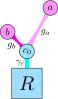
\includegraphics[width=0.3\linewidth, draft=false]{phog/three_mode}
\caption{\label{fig:phog_three_mode} Three-mode model of PhoG device. Two bosonic modes, $a$ and $b$, are each coupled to a third mode, $c_0$. Mode $c_0$ is then strongly coupled to Markovian reservoir $R$ via linear loss $\left(\hat{A} = \hat{a}\right)$ with decay rate $\gamma_c$. }
\end{figure}

The Lindblad equation describing this three-mode model is
\begin{equation}\label{eqn:phog_lindblad_three_mode_model}
\ddt \rho_3 = - i \left[ \hat{H}_3, \rho_3\right] + \left[ \gamma_L \mathcal{L}\left(\hat{a}\right) + \gamma_L \mathcal{L}\left(\hat{b}\right) + \gamma_c \mathcal{L}\left(\hat{c}_0\right)\right] \rho_3
\end{equation}
where the subscript $3$ denotes that we are dealing with this three-mode model. We have taken modes $a$ and $b$ to be coupled to independent Markovian reservoirs with rate $\gamma_L$ which models the conventional linear loss. The Hamiltonian is taken to be $\hat{H}_3 = \hat{H}_3^{\text{int}} + \hat{H}_3^{\text{Kerr}}$, where
\begin{align}\label{eqn:phog_three_mode_hamiltonian}
\hat{H}_3^{\text{int}} &= g_a \hat{a}^\dagger \hat{c}_0 + g_b \hat{b}^\dagger \hat{c}_0 + \hc \notag \\
%
\hat{H}_3^{\text{Kerr}} &= \frac{U}{2} \sum_{x} \hat{x}^\dagger \hat{x}^\dagger \hat{x} \hat{x} \qq{with} \hat{x} \in \left\{\hat{a}, \hat{b}, \hat{c}_0\right\}.
\end{align}
The interaction Hamiltonian $\hat{H}_3^{\text{int}}$ describes linear coupling between modes, while the Kerr Hamiltonian $\hat{H}_3^{\text{Kerr}}$ describes the self-Kerr interaction (self-phase modulation)% Check that these are indeed equivalent
on each mode. This Hamiltonian may be realised, for example, by evanescently coupled waveguides in a $\chi^{\left(3\right)}$ glass. The $U$ is the Kerr nonlinear interaction constant, and we will relate this to glass properties in Sec.~\MT{X} below.

The three-mode model Eq.~\ref{eqn:phog_lindblad_three_mode_model}, while a physically useful starting point for building a system which accurately simulates NCL, is as yet too complicated to difficult to analyse, either analytically or using the numerical methods which proved useful for the single mode model in Secs.~\ref{sec:phog_single_mode_model},~\ref{sec:phog_including_loss}. \MT{I should have an appendix where I discuss the numerical methods which I used in that section.}

We may reduce the complexity of Eq.~\ref{eqn:phog_lindblad_three_mode_model} by assuming that the decay rate $\gamma_c$ of mode $c_0$ into the reservoir $R$ is large enough that mode $c_0$ completely decays on a much faster timescale than modes $a, b$. This will allow for adiabatic elimination of mode $c_0$ via the methods described in Appendix.~\ref{appendix:adiabatic_elimination}. We identify
\begin{align}
H^{\left(0, 0\right)} &= \frac{U}{2} \sum_{x \in \left\{a, b\right\}} x^{\dagger 2} x^2 \notag \\
%
H^{\left(0, 1\right)} &= g_a a^\dagger c_0 + g_b b^\dagger c_0 \notag \\
%
H^{\left(0, 2\right)} = 0
\end{align}
and so, substituting into Eq.~\ref{eqn:adiabatic_elimination}, we arrive at
\begin{equation}\label{eqn:phog_two_mode_model_deriv}
\ddt \rho_2 = - i \left[\frac{U}{2} \sum_{x \in \left\{a, b\right\}} x^{\dagger 2} x^2, \rho_2\right] + \frac{4 G^2}{\gamma_c} \mathcal{L}\left(\frac{g_a a + g_b b}{G} \right)\rho_2 + \gamma_L \left(\mathcal{L}\left(a\right) + \mathcal{L}\left(b\right)\right)\rho_2,
\end{equation}
and so we have reduced our three-mode model to a two-mode system involving only modes $a, b$. Introducing the following collective symmetric and antisymmetric modes

\begin{align}\label{eqn:phog_rotation}
\hat{s}_+ &= \frac{1}{G} \left(g_a \hat{a} + g_b \hat{b}\right) \qq{symmetric}  \notag \\
%
\hat{s}_- &= \frac{1}{G} \left(g_a \hat{b} - g_b \hat{a}\right) \qq{antisymmetric}
\end{align}
with $G = \sqrt{ g_a^2 + g_b^2 }$ required to ensure that $\hat{s}_-, \hat{s}_+$ obey the same bosonic commutation relations as $\hat{a}, \hat{b}$. Rewriting Eq.~\ref{eqn:phog_two_mode_model_deriv} in terms of these new modes we arrive at our two-mode model
\begin{equation}\label{eqn:phog_lindblad_two_mode_model}
\ddt \rho_2 = - i \left[ \hat{H}_2, \rho_2 \right] + \left[ \gamma_L \mathcal{L}\left(\hat{s}_-\right) + \left(\Gamma + \gamma_L\right) \mathcal{L}\left(\hat{s}_+\right) \right] \rho_2
\end{equation}
where the subscript $2$ denotes that each quantity is for this two-mode model, and we have defined $\Gamma = 4 G^2 / \gamma_c$. The Hamiltonian $\hat{H}_2$ takes the form $\hat{H}_2 = \hat{H}_2^{\text{self}} + \hat{H}_2^{\text{int}}$, with
\begin{align}
H_2^{\text{self}} = \varsigma_1\left(n_+^2 + n_-^2\right) + \varsigma_2 n_+ n_- + \varsigma_3\left(n_+ + n_-\right) \notag \\
%
H_2^{\text{int}} = \varsigma_4 \left(s_+^\dagger s_-\right)^2 + \varsigma_5 s_+^\dagger s_- \left(n_- - n_+ - 1\right) + \hc
\end{align}
where $n_{\pm} = s_{\pm}^\dagger s_\pm$ and our $\varsigma$ coefficients are
\begin{align}
\varsigma_1 = \frac{U}{2 G^4} \left(g_a^4 + g_b^4\right), \; \varsigma_2 = \frac{4 U}{G^4} \left(g_a g_b\right)^2, \notag \\
%
\varsigma_3 = \frac{\varsigma_2}{4} - \frac{U}{2}, \; \varsigma_4 = \frac{\varsigma_2}{4}, \; \varsigma_5 = \frac{U}{G^4} g_a g_b \left(g_a^2 - g_b^2\right).
\end{align}
Our two-mode model is depicted in Fig.~\ref{fig:phog_two_mode_model} where we see that mode $s_+$ decays into reservoir $R$ with decay rate $\Gamma + \gamma_L$. In the absence of linear loss, $\gamma_L=0$, mode $s_-$ will decay only vicariously through $s_+$, and the coupling between modes is proportional to nonlinearity parameter $U$. In a linear system, $U = 0$, the antisymmetric mode $s_-$ will not decay and so we identify it as the dark mode of the system which is considered e.g. in Ref.~\MT{Twamley paper}.


\begin{figure}[htp]
\centering
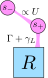
\includegraphics[width=0.3\linewidth, draft=false]{phog/two_mode}
\caption{\label{fig:phog_two_mode_model} Two-mode model of the PhoG device. Having adiabatically eliminated mode $c_0$ from the three-mode model (Fig.~\ref{fig:phog_three_mode}) and rotated to collective basis $s_-, s_+$ using Eqs.~\ref{eqn:phog_rotation} we see that mode $s_-$ will only decay into $R$ by first decaying into $s_+$. The linear coupling between $s_-$ and $s_+$ is proportional to $U$, and so for a linear system $U=0$ mode $s_-$ cannot decay into $R$. $\Gamma = 4 G^2 / \gamma_L$.}
\end{figure}


\MT{Some chat about simulating the two-mode model.}


However, even two bosonic modes are computationally very challenging to simulate when large photon numbers are required \MT{comment about hilbert-space-size-scaling}, and so we seek to adiabatically eliminate mode $s_+$ from the system, which will leave us with an equation for $s_-$ only. 

Let us assume that the decay rate $\Gamma + \gamma_L$ is the dominating decay rate of the two-mode model, and that mode $s_+$ decays to its steady state much quicker than the dynamics of $s_-$. Then applying the adiabatic elimination method described in Appendix~\ref{appendix:adiabatic_elimination} we identify

\begin{align}
H^{\left(0, 0\right)} &= \varsigma_1 n_-^2 + \varsigma_3 n_- \notag \\ 
%
H^{\left(0, 1\right)} &= \varsigma_5 s_-^\dagger n_- \notag \\
%
H^{\left(0, 2\right)} &= \varsigma_4 s_-^{\dagger 2}
\end{align}
and so

\begin{equation}\label{eqn:phog_single_mode_deriv}
\ddt \rho_1 = - i \left[\hat{H}_1, \rho_1\right] + \left\{\gamma_L \mathcal{L}\left(s_-\right) + \gamma_2 \mathcal{L}\left(s_-^2\right) + \gamma_3 \mathcal{L}\left(\ncl\right) \right\}\rho_1
\end{equation}
where we have used the commutator to write $n_- s_- \rightarrow \ncl$, and where
\begin{equation}
\gamma_2 = \frac{4 U^2 \left(g_a g_b\right)^4}{G^8 \left(\Gamma + \gamma_L\right)} \qq{and} \gamma_3 = \frac{4 U^2 \left(g_a g_b\right)^2}{G^8 \left(\Gamma + \gamma_L\right)}\left(g_a^2 - g_b^2\right)^2.
\end{equation}

\noindent We see that Eq.~\ref{eqn:phog_single_mode_deriv} matches Eq.~\ref{eqn:phog_full_single_mode} except for the addition of the Hamiltonian $\hat{H}$ which does not affect the photon-number statistics. 

To summarise, we have reduced the three-mode model (Eq.~\ref{eqn:phog_lindblad_three_mode_model}, Fig.~\ref{fig:phog_three_mode}) to a single-mode model (Eqs.~\ref{eqn:phog_full_single_mode}
,~\ref{eqn:phog_single_mode_deriv}, Fig.~\ref{fig:phog_single_mode}) via two sequential adiabatic eliminations of modes $c_0$ and $s_+$, which rapidly decayed into reservoir $R$. In essence, the behaviour of the antisymmetric collective mode $s_-$ in the three-mode model simulates behaviour of a single mode undergoing both nonlinear coherent loss, two-photon loss and single-photon loss, which were all considered in Secs.~\ref{sec:phog_single_mode_model}~\ref{sec:phog_including_loss}. The combination of Kerr nonlinearity, linear coupling and single-photon loss allows for the effective NCL decay operator to be constructed.

The effective decay rates in this single-mode model explicity depend on coupling constants $g_a, g_b$ (Fig.~\ref{fig:phog_three_mode}, Eq.~\ref{eqn:phog_three_mode_hamiltonian}). We see for example that in the limit of symmetric coupling $g_a = g_b$, $\gamma_3 = 0$ and there will be no NCL for mode $s_-$. Large $\gamma_3$ can be obtained however for strong asymmetry $g_a \gg g_b$ or $g_b \gg g_a$. Since it is NCL which drives $\rho$ most effectively towards highly sub-Poissonian states we will seek to maximise $\gamma_3$.


%\MT{I can't do this until I have motivated the best choice of $g_a, g_b$.}
%We are finally able to give motivation for the choices of $\gamma_2=0.0005, \gamma_3=0.002$ used in Sec.~\ref{sec:phog_summary_ncl_effects} as the 











\bibliographystyle{unsrt} 
%\bibliography{Thesis}


\appendix
%\include{chapters/larger_alphabets}
%\include{chapters/coherent_noisy_channel}
%%
% Q: do I need to reference Shchesnovich2011? Or other places?
%
%


\chapter{PhoG: Adiabatic elimination}\label{appendix:adiabatic_elimination}

In this appendix we will derive Eq.~\ref{eqn:adiabatic_elimination} which is used in Sec.~\ref{sec:phog_three_mode_model} to simplify the analytical description of a multi-mode bosonic system when one of the modes takes its steady-state. Our analysis will use notation following Ref.~\cite{Shchesnovich2011}. 

Consider a system involving a highly lossy bosonic mode, $c$. We assume that $c$ decays into a Markovian reservoir with decay rate $\gamma$, and that the system contains additional modes with possible losses, couplings and nonlinearities. 

After $t \gg 1/\gamma$ the mode $c$ is empty, and it is assumed that this timescale is much faster than all other timescales in the system. Then, for $t \gg 1/\gamma$ the mode $c$ can be assumed to be in its steady-state and so, for example, $\ddt \hat{c} = 0$. This will be used in order to simplify the description of our original system.

The Lindblad master equation for our entire system is

\begin{equation}
\ddt \rho = - i \left[ \hat{H}, \rho \right] + \gamma \mathcal{L}\left[\hat{c}\right] \rho + \Gamma_j\mathcal{L}\left[f\left(\hat{a}_j\right)\right] \rho,
\end{equation}
where $\rho$ is the density matrix describing the entire system and $\hat{H}$ is the system's Hamiltonian, on which we will later derive some restrictions. The term proportional to  $\gamma$ denotes strong loss of mode $c$ into the reservoir, and the term in $\Gamma$ denotes potential other sources of loss which do not affect $c$. We shall ignore terms in $\Gamma_j$ until the very last step, since they do not affect our analysis and will always be present.

It is easiest to proceed in Heisenberg picture, and so we transform to the adjoint master equation \cite{Breuer2002} which describes the evolution of an arbitrary operator $\hat{A}$

\begin{equation}\label{eqn:appendix_phog_adjoint_start}
\ddt \hat{A} = i \left[ \hat{H}, \hat{A} \right] + \gamma \mathcal{L}\left[\hat{c}^\dagger \right] \hat{A} + \Gamma_j \mathcal{L} \left[ f\left(\hat{a}_j\right)^\dagger\right] \hat{A},
\end{equation}
and expand $\hat{H}$ and $\hat{A}$ in terms of normal-ordered powers of creation and annihilation operators of the lossy mode
\begin{align}
&\hat{H} = \sum_{p, q = 0}^{\infty} \hat{H}^{\left(p, q\right)} \left(\hat{c}^\dagger\right)^p \hat{c}^q, \label{eqn:appendix_phog_H_expand}  \\
%
&\hat{A} = \sum_{p, q = 0}^{\infty} \hat{A}^{\left(p, q\right)}\left(t\right) \left(\hat{c}^\dagger \right)^p \hat{c}^q . \label{eqn:appendix_phog_A_expand}
\end{align}
Operators $\hat{H}^{\left(p, q\right)}, \hat{A}^{\left(p, q\right)}$ are, in general, operators acting on the remaining modes of the system. Let us take Eqs.~\ref{eqn:appendix_phog_H_expand},~\ref{eqn:appendix_phog_A_expand} and substitute into Eq.~\ref{eqn:appendix_phog_adjoint_start}. Grouping terms in $\hat{c}^\dagger, \hat{c}$ we see that 

\begin{align}
\ddt A^{\left(m, n\right)}\left(t\right) c^{\dagger m} c^n = i \sum_{p, q, k, l} &\left(H^{\left(k, l\right)} A^{\left(p, q\right)}\left(t\right) c^{\dagger k} c^{l} c^{\dagger p} c^q \right. \notag \\
&\left.- A^{\left(p, q\right)}\left(t\right) H^{\left(k, l\right)} c^{\dagger p} c^q c^{\dagger k} c^l\right)
%
+ \qq{terms in $\gamma$, $\Gamma$.}&
\end{align}
We have dropped hats from operators for ease of notation. Relabelling dummy indices,
\begin{equation}\label{eqn:appendix_phog_Apq}
\ddt A^{\left(p, q\right)}\left(t\right) c^{\dagger p} c^q = i \sum_{p, q, k, l} F\left(p, q, k, l; t\right) c^{\dagger p} c^{q} c^{\dagger k} c^l + \qq{terms in $\gamma$, $\Gamma$},
\end{equation}
where
\begin{equation}
F\left(p, q, k, l; t\right) = H^{\left(k, l\right)} A^{\left(p, q\right)}\left(t\right) - A^{\left(p, q\right)}\left(t\right) H^{\left(k, l\right)}. \notag
\end{equation}

\noindent The differential equation for $A^{\left(0, 0\right)}$ is such that there are no operators in mode $c$ remaining on the right hand side of Eq.~\ref{eqn:appendix_phog_Apq}. Clearly this occurs when $p=q=k=l=0$. It can also occur for other values of $p, q, k, l$, owing to constant terms appearing via the commutators of $\hat{c}$ operators. Additionally, since the Lindblad operator $\mathcal{L}$ is second-order in $\hat{c}$ we can see immediately that there will be no terms proportional to $\gamma$ in the equation for $A^{\left(0, 0\right)}$. 

Writing Eq.~\ref{eqn:appendix_phog_Apq} in normal order using the commutator,
\begin{align}
\ddt A^{\left(p, q\right)}\left(t\right) c^{p, \dagger} c^q = i \sum_{p, q, k, l} &\left( F\left( p, q, k, l;t\right) c^{\dagger p} c^{\dagger k} c^q c^l \right. \notag \\
&\left.+ F\left(p, q, k, l;t\right)  \left[ c^{q}, c^{\dagger k}\right] c^{\dagger p} c^l \right),
\end{align}
we observe that additional contributions to $A^{\left(0, 0\right)}$ are possible when $p=0, l=0$ but $q, k \ne 0$ provided that the commutator $\left[ c^q, c^{\dagger k}\right]$ contains a constant term. We observe

\begin{align}\label{eqn:phog_appendix_commutator}
\left[ c, c^\dagger \right] &= 1, \notag \\
%
\left[ c^2, c^{\dagger 2} \right] &= 4 c^\dagger c + 2, \notag \\
%
\left[ c^3, c^{\dagger 3} \right] &= 9 c^\dagger c^\dagger c c + 18 c^\dagger c + 6 ,\notag \\
%
&\vdots
\end{align}
while commutators with $q \ne k$ cannot give a constant term. 

For ease, and because the largest terms considered in Ch.~\ref{chapter:phog} are of the form $c^\dagger c^\dagger c c$ we will restrict ourselves to $0 \le q, k \le 2$. This gives

\begin{equation}
\ddt A^{\left(0, 0\right)}\left(t\right) = i \left( \left[ H^{\left(0, 0\right)}, A^{\left(0, 0\right)}\right] + F\left(0, 1, 1, 0\right) + 2 F\left(0, 2, 2, 0\right)\right), \notag
\end{equation}
and so 
\begin{align}\label{eqn:ddt_a00}
\ddt A^{\left(0, 0\right)}\left(t\right) = i  &\left(\left[ H^{\left(0, 0\right)}, A^{\left(0, 0\right)}\right] + H^{\left(0, 1\right)} A^{\left(1, 0\right)} - A^{\left(0, 1\right)} H^{\left(1, 0\right)} \right. \notag \\
%
&+\left. 2 H^{\left(0, 2\right)} A^{\left(2, 0\right)} - 2 A^{\left(0, 2\right)} H^{\left(2, 0\right)} \right).
\end{align}

\noindent Let us return to Eq.~\ref{eqn:appendix_phog_adjoint_start} and substitute Eq.~\ref{eqn:appendix_phog_A_expand} into the $\gamma$ term. By rearranging into normal order we arrive at
\begin{equation}
\gamma \mathcal{L}\left[\hat{c}^\dagger\right] \hat{A} \rightarrow - \gamma \sum_{p, q}\frac{\left(p + q\right)}{2} \hat{A}^{\left(p, q\right)} \hat{c}^{\dagger p} \hat{c}^q,
\end{equation} %TODO: make sure that I know how to do this for the viva.
and so for $t \gg 1/\gamma$ we may approximate the evolution of $\hat{A}^{\left(p, q\right)}$ by
\begin{equation}
\ddt A^{\left(p, q\right)} \approx i \left[ H^{\left(p, q\right)}, A^{\left(0, 0\right)}\right] - \frac{\gamma \left(p + q\right)}{2} A^{\left(p, q\right)},
\end{equation}
since $A^{\left(p, q\right)}$ is dominated by the decay. Assuming that $t$ is such that $A^{\left(p, q\right)}$ has reached its steady-state we set $\ddt A^{\left(p, q\right)} = 0$ and so
\begin{equation}
A^{\left(p, q\right)} \left(t\right) \approx \frac{2 i}{\gamma \left(p + q\right)} \left[H^{\left(p, q\right)}, A^{\left(0, 0\right)}\left(t\right)\right],
\end{equation}
provided that $p \ne 0$ or $q \ne 0$. By substituting this equation for $A^{\left(p, q\right)}$ into Eq.~\ref{eqn:ddt_a00}, we finally arrive at

\begin{equation}
\ddt A^{\left(0, 0\right)} = i \left[ H^{\left(0, 0\right)}, A^{\left(0, 0\right)}\right] + \frac{4}{\gamma} \sum_{p = {1, 2}} \mathcal{L}\left[ H^{\left(0, p\right)} \right] A^{\left(0, 0\right)} + \Gamma_j \mathcal{L}\left[a_j\right] \rho. %Can I just stick the extra loss term here? Is it affected by the adiabatic elimination at all?
\end{equation}
Transforming back to our master equation in Lindblad form,
\begin{equation}\label{eqn:adiabatic_elimination}
\ddt \rho = - i \left[ H^{\left(0, 0\right)}, \rho\right] + \frac{4}{\gamma} \sum_{p = 1, 2} \mathcal{L} \left[H^{\left(0, p\right)\dagger}\right] \rho + \Gamma_j \mathcal{L}\left[a_j\right] \rho.
\end{equation}
This Eq.~\ref{eqn:adiabatic_elimination} is our key equation for performing the adiabatic elimination of the highly lossy mode\footnote{Mode $\hat{c}$ in Chapter~\ref{chapter:phog}.}. The recipe to apply it to a general system is to identify the $H^{\left(0, 0\right)}$ and $H^{\left(0, p\right)}$ terms, which can take arbitrary form, and then substitute them into Eq.~\ref{eqn:adiabatic_elimination}. The only requirement for the use of Eq.~\ref{eqn:adiabatic_elimination} is that $\hat{H}$ must have its largest term in lossy mode $c$ of the form $\hat{c}^\dagger \hat{c}^\dagger \hat{c} \hat{c}$, i.e. two creation and two annihilation operators. More general forms of Eq.~\ref{eqn:adiabatic_elimination} may be considered by continuing our analysis to higher-order commutators $\left[ \hat{c}^n, \hat{c}^{\dagger n}\right]$ which has constant term $n!$, allowing for different maximum combinations of $\hat{c}$ operators 


\chapter{PhoG: Numerical methods}\label{appendix:phog_numerical_methods}

In this appendix we will briefly overview the numerical methods which are used in Part $2$ of this Thesis. The first two, Secs.~\ref{appendix:direct_integration},~\ref{appendix:monte_carlo} are standard methods for handling the Lindblad master equation with much written about them elsewhere \MT{cite}, and so we will discuss them only in passing. The final two methods, mean-field and linearization, Secs.~\ref{appendix:mean-field},~\ref{appendix:single_mode_linear},~\ref{appendix:multi_mode_linear}, are discussed at length in the main body of the Thesis, Sec.~\ref{sec:phog_multi_mode}, and so we will just reproduce the final systems of equations in this Appendix.

\section{Direct integration}\label{appendix:direct_integration}

The dynamics of a quantum system coupled to a reservoir is governed by the Lindblad equation
\begin{equation}\label{eqn:appendix_lindblad}
\ddt \rho = - i \left[ \hat{H}, \rho \right] + \sum_n \left(\hat{C}_n \rho \hat{C}_n^\dagger - \frac{1}{2} \hat{C}_n^\dagger \hat{C}_n \rho - \frac{1}{2} \rho \hat{C}_n^\dagger \hat{C}_n \right)
\end{equation}
where $\hat{H}$ acts only on $\rho$ and $\hat{C}_n$ are the collapse operators governing decay into the reservoir. Here we take $\hat{C}_n = \sqrt{\gamma_n} \hat{A}_n$ where $\hat{A}_n$ is an operator acting on $\rho$, and is the operator through which $\rho$ couples to the reservoir in the original system-reservoir Schr{\"o}dinger equation. The derivation of this Lindblad equation including requisite approximations is discussed extensively in many classic texts such as Refs.~\cite{Breuer2002, Carmichael1999}. 

There are many routes which one can take to solve Eq.~\ref{eqn:appendix_lindblad}. One such approach is to interpret $\rho$, $\hat{H}$ and $\hat{C}_n$ as matrices. Let our underlying Hilbert-space be denoted $\mathcal{H}$ and have dimension $\dims$. Then $\rho$, $\hat{H}$ and $\hat{C}_n$ each have dimension $\dims$ and may be interpreted as a matrices in $M_{\dims \times \dims}\left(\mathbb{C}\right)$. The Lindblad equation~\ref{eqn:appendix_lindblad} may be interpreted as a coupled system of $\dims^2$ first-order ODEs. This system can then be solved via an appropriate numerical method \MT{cite something - advanced engineering mathematics? Or numerical methods book?}, the efficiency and power of which will depend strongly on the choices of $\hat{H}$, $\hat{C}_n$ and initial condition $\rho\left(0\right)$.

In this Thesis we use the open-source QuTiP package\footnote{QuTiP version $4.4.1$; Numpy version $1.16.4$; Scipy version $1.3.1$; Cython version $0.29.13$; Matplotlib version $3.1.0$; Python version $3.7.4$} \cite{qutip2} in Python to perform such numerical solutions. Direct integration of the ODE system is performed using \code{qutip.mesolve} command, with the actual integration performed by \code{scipy.integrate.ode} \MT{cite}. 

On a standard home-use laptop\footnote{Intel(R) Core(TM) i$5-3230$M CPU $@ 2.60$~GHz; $8.00$~GB RAM} a single-mode system with $\dims = 35$, $\rho\left(0\right)$ a coherent state with $\alpha = 3.0$, decay rate $\gamma = 8.0$, collapse operator $\hat{a}$ and free Hamiltonian $\hat{H} = \omega \hat{a}^\dagger \hat{a}$ with $\omega = 1.0$ can be solved in $58.3$~ms $\pm 5.65$~ms\footnote{Timed via iPython \code{\%timeit} magic command.}. Setting $\dims = 50$ takes $195 \pm 9.8$~ms, $\dims = 200$ takes $2.76$~s $\pm 129$~ms.

However, using collapse operator $\ncl$ increases the computational power required, and $\dims = 10$ takes $341 \pm 77.2$~ms, $\dims = 35$ takes over $100$~s, and $\dims=100$ takes $18$~minutes. Larger $\dims$ are intractable. We see then that this approach is highly dependent on both the form of $\hat{H}, \hat{C}_n$ and the Hilbert-space size. Indeed, a Hilbert space size $\dims$ yields $\dims^2$ coupled ODEs to solve. 

The coherent state must be defined in QuTiP specifying the ``analytic" option to \code{qutip.coherent\_dm}, which ensures that $\dyad{\alpha}$ uses the expression Eq.~\ref{eqn:intro_coherent_state}. The default option ``operator" instead finds the eigenstate of collapse operator $\hat{a}$. As $\dims \rightarrow \infty$ the two forms of coherent state become equivalent, but for small $\dims$ they can differ significantly. We have found that the analytic form gives much more accurate behaviour in the parameter ranges considered. Since the coherent state lives on an infinite-dimensional Hilbert space, care must be taken to choose $\dims$ sufficiently large that no ill effects are introduced from the truncation to a finite-sized one. A good rule-of-thumb is to pick
\begin{equation*}
\dims \ge \lceil 2 \alpha^2 \rceil
\end{equation*}
which ensures that the coherent state Eq.~\ref{eqn:appendix_coherent_state_truncated} is correctly normalized and a good approximation of the full Eq.~\ref{eqn:intro_coherent_state}. \MT{add truncated coherent state}. In any case, in all simulations we include built-in checks of state normalization which indicate when $\dims$ must be increased.

\MT{mention about scaling with number of modes}

\MT{integrate this section into the thesis body. Which graphs and quantities did I calculate via direct integration?}

\section{Quantum Monte-Carlo}\label{appendix:monte_carlo}
We have seen that direct integration of Eq.~\ref{eqn:appendix_lindblad} requires a system of $\dims^2$ coupled ODEs to be simultaneously solved. This is doable in the limit of small $\dims$, but quickly becomes difficult as $\dims$ increases. An alternative approach does not solve a matrix differential equation, rather a vector one, and so instead scales with $\dims$.

We will briefly outline the quantum monte-carlo approach and then discuss its implementation and use in this Thesis.



\section{Linearized single-mode model}\label{appendix:single_mode_linear}
By applying the linearization approximations derived in Sec.~\ref{sec:linearization} to the system of coupled ODEs derived from single-mode Lindblad equation~\ref{eqn:phog_single_mode_deriv} we arrive at the following closed system of ODEs:


\begin{align}\label{eqn:expectations_linear_first}
%
%a
%
\partial_t\langle s_- \rangle &= c_1 \langle s_- \rangle + c_2 \left(\langle s_-^\dagger \rangle \langle s_-^2 \rangle + 2 \langle s_- \rangle \langle n_-\rangle - 2 \langle s_-^\dagger \rangle \langle s_- \rangle^2\right) \notag \\
%
&-\frac{\gamma_3}{2}\left(
6 \langle s_-^\dagger \rangle \langle n_- \rangle \langle s_-^2\rangle + 3 \langle s_- \rangle \langle s_-^{\dagger 2} \rangle \langle s_-^2 \rangle \right. \notag \\
%
&+ 6 \langle s_- \rangle \langle n_- \rangle^2 - 2 \langle s_-^{\dagger 2} \rangle \langle s_- \rangle^3 - 12 \langle n_- \rangle \langle s_-^\dagger \rangle \langle s_- \rangle^2 \notag \\
%
&\left. - 6 \langle s_-^2 \rangle \langle s_-^\dagger \rangle^2 \langle s_- \rangle + 6 \langle s_-^\dagger \rangle^2 \langle s_- \rangle^3\right)
\end{align}
\begin{align}
%
% ad
%
\partial_t\langle s_-^\dagger \rangle &= c_1^* \langle s_-^\dagger \rangle + c_2^* \left(\langle s_- \rangle \langle s_-^{\dagger 2} \rangle + 2 \langle s_-^\dagger \rangle \langle n_- \rangle - 2 \langle s_-^\dagger \rangle^2\langle s_- \rangle \right) \notag \\
%
&-\frac{\gamma_3}{2}\left(6 \langle s_- \rangle \langle n_- \rangle \langle s_-^{\dagger 2}\rangle + 3 \langle s_-^\dagger \rangle \langle s_-^2 \rangle \langle s_-^{\dagger 2}\rangle \notag \right. \notag \\
%
&+ 6 \langle s_-^\dagger \rangle \langle n_-\rangle^2 - 2 \langle s_-^2 \rangle \langle n_-^3\rangle - 12 \langle n_- \rangle \langle s_- \rangle \langle s_- \rangle^2 \notag \\
%
&\left. - 6 \langle s_-^{\dagger 2} \rangle \langle s_- \rangle^2 \langle s_-^\dagger \rangle + 6 \langle s_-^{\dagger 3} \rangle \langle s_- \rangle^2 \right)
\end{align}
\begin{align}
%
% aa
%
\partial_t\langle s_-^2 \rangle &= c_3 \langle s_- s_- \rangle + c_4 \left( 3 \langle n_- \rangle \langle s_-^2 \rangle  - 2 \langle s_-^\dagger \rangle \langle s_- \rangle^3 \right) \notag \\
%
&- \gamma_3 \left( 3 \langle s_-^{\dagger 2}\rangle \langle s_-^2\rangle^2 + 12 \langle n_- \rangle^2 \langle s_-^2\rangle - 2 \langle s_-^{\dagger 2}\rangle \langle s_- \rangle^4 \right. \notag \\
%
& - 12 \langle s_-^2 \rangle \langle s_-^{\dagger}\rangle^2 \langle s_- \rangle^2 - 16 \langle n_- \rangle \langle s_-^\dagger \rangle \langle s_- \rangle^3 \notag \\
%
&\left. + 16 \langle s_-^\dagger \rangle^2 \langle s_- \rangle^4 \right)
\end{align}
\begin{align}
%
% adad
%
\partial_t\langle s_-^{\dagger^2} \rangle &= c_3^* \langle s_-^{\dagger 2}\rangle + c_4^* \left(3 \langle s_-^{\dagger 2} \rangle \langle n_- \rangle - 2 \langle s_-^\dagger \rangle^3 \langle s_- \rangle \right) \notag \\
%
&- \gamma_3 \left(3 \langle s_-^{\dagger 2} \rangle^2 \langle s_-^2 \rangle + 12 \langle s_-^{\dagger 2} \rangle \langle n_- \rangle^2 - 2\langle s_-^2 \rangle \langle s_-^\dagger \rangle^4 \right. \notag \\
%
&\left. - 21 \langle s_-^{\dagger 2}\rangle \langle s_-^\dagger\rangle^2 \langle s_- \rangle^2 - 16 \langle n_- \rangle \langle s_-^\dagger \rangle^3 \langle s_-\rangle \right. \notag \\
%
& \left.+ 16 \langle s_-^\dagger\rangle^4 \langle s_- \rangle^2 \right)
\end{align}
\begin{align}\label{eqn:expectations_linear_last}
%
% ada
%
\partial_t \langle n_- \rangle &= - \gamma_1 \langle n_- \rangle + c_5 \left( \langle s_-^{\dagger 2} \rangle \langle s_-^2 \rangle + 2 \langle n_- \rangle^2 - 2 \langle s_-^\dagger \rangle^2 \langle s_- \rangle^2 \right) \notag \\
%
&- \gamma_3 \left( 9 \langle s_-^{\dagger 2} \rangle \langle n_-  \rangle \langle s_-^2\rangle + 6 \langle n_-\rangle^3  - 6 \langle s_-^{\dagger 2}\rangle \langle s_-^\dagger \rangle \langle s_- \rangle^3 \right. \notag \\
%
& - 18 \langle n_- \rangle \langle s_-^\dagger \rangle^2 \langle s_- \rangle^2 - 6 \langle s_-^2 \rangle \langle s_-^\dagger \rangle^3 \langle s_- \rangle \notag \\
%
& \left. + 16 \langle s_-^\dagger \rangle^3 \langle s_-\rangle^3 \right)
\end{align}
with $n_- = s_-^\dagger s_-$.

This system is solved numerically for $\langle s_- \rangle$, $\langle s_-^\dagger \rangle$, $\langle s_-^2\rangle$, $\langle s_-^{\dagger 2}\rangle$, $\langle n_-\rangle$ and the results are shown as dashed lines in Fig.~\ref{fig:phog_single_mode_linearization}.


\section{Linearized multi-mode model}\label{appendix:multi_mode_linear}
We will derive a linearized and closed system of coupled differential equations capable of modelling the multi-mode PhoG device. In fact, our equations will be capable of modelling any collection of coupled modes with on-site Kerr nonlinearity and Markovian reservoirs. Our starting Lindblad equation is Eq.~\ref{eqn:phog_multi_mode}

\begin{equation}
\ddt \rho = - i \left[\hat{H}, \rho\right] + \gamma_1 \left[\mathcal{L}\left(\hat{a}_1\right) + \mathcal{L}\left(\hat{a}_2\right) + \sum_{j=3}^{N+2} \mathcal{L}\left(\hat{a}_j\right) \right] \rho
\end{equation}
where we here take $\hat{H} = \hat{H}^{\text{Coupling}} + \hat{H}^{\text{Kerr}}$. In this Appendix we label all modes as $\hat{a}_k$, with the subscript denoting which mode in the PhoG device is meant. In particular, $a_1 \leftrightarrow a$, $a_2 \leftrightarrow b$, and $a_{k \ge 3} \leftrightarrow c_{k-3}$ in the main body. The Hamtiltonian is
\begin{align}
\hat{H}^{\text{Kerr}} = \frac{U}{2} \sum_{x} \hat{x}^\dagger \hat{x}^\dagger \hat{x} \hat{x} \qq{} x \in \left\{a, b, c_j\right\}\; 0 \le j \le N
%
\hat{H}^{\text{Coupling}} = \sum_{k, l} \mathcal{G}_{k, l}\left(\hat{a}_k^\dagger \hat{a}_l + \hat{a}_l^\dagger \hat{a}_k \right)
\end{align}
where we have introduced a "coupling matrix" $\mathcal{G}$ which contains all information relating to the linear coupling between modes of our system. Coupling matrix element $\mathcal{G}_{j, p}$ denotes the coupling strength between modes $j$ and $p$, and $\mathcal{G}_{j, p} = 0$ if the modes are not coupled to each other, which is the case for most pairs $\left(j, p\right)$. We display some example coupling matrices below.
\subsection{Example coupling matrices $\mathcal{G}$}
\begin{figure}[htp]
\begin{minipage}{.4\textwidth}
\[
\mathcal{G} = 
\begin{bmatrix}
0 & \highlight{g} & 0 & 0 & \dots & 0 & 0 & 0 \\
\highlight{g} & 0 & \highlight{g} & 0 & \dots & 0 & 0 & 0 \\
0 & \highlight{g} & 0 & \highlight{g} & \dots & 0 & 0 & 0  \\
0 & \vdots & \vdots & \vdots & \ddots & \vdots & \vdots & 0 \\
0 & 0 & 0 & 0 & \dots & 0 & \highlight{g} & 0 \\
0 & 0 & 0 & 0 & \dots & \highlight{g} & 0 & \highlight{g} \\
0 & 0 & 0 & 0 & \dots & 0 & \highlight{g} & 0
\end{bmatrix}
\]
\end{minipage}
\begin{minipage}{.5\textwidth}
\centering
\includegraphics[width=0.3\textwidth, draft=false]{phog/bosonic_line_vertical}
\end{minipage}
\caption{\label{fig:coupline}Line of modes}
\end{figure}



\begin{figure}[htp]
\begin{minipage}{.4\textwidth}
\[
\mathcal{G} = 
\begin{bmatrix}
0 & 0 & \highlight{g1} & 0 & 0 & 0 & \dots & 0 & 0 & 0 \\
0 & 0 & \highlight{g2} & 0 & 0 & 0 & \dots & 0 & 0 & 0 \\
\highlight{g1} & \highlight{g2} & 0 & \highlight{g3} & 0 & 0 & \dots & 0 & 0 & 0 \\
0 & 0 & \highlight{g3} & 0 & \highlight{g3} & 0 & \dots & 0 & 0 & 0 \\
0 & 0 & 0 & \highlight{g3} & 0 & \highlight{g3} & \dots & 0 & 0 & 0 \\
0 & 0 & 0 & 0 & \highlight{g3} & 0 & \dots & 0 & 0 & 0  \\
0 & \vdots & \vdots & \vdots & \vdots & \vdots & \ddots & \vdots & \vdots & 0 \\
0 & 0 & 0 & 0 & 0 & 0 & \dots & 0 & \highlight{g3} & 0 \\
0 & 0 & 0 & 0 & 0 & 0 & \dots & \highlight{g3} & 0 & \highlight{g3} \\
0 & 0 & 0 & 0 & 0 & 0 & \dots & 0 & \highlight{g3} & 0 
\end{bmatrix}
\]
\end{minipage}
\begin{subfigure}{.4\textwidth}
\centering
\includegraphics[width=0.3\textwidth, draft=false]{phog/bosonic_chain_phog_vertical}
\end{subfigure}
\caption{\label{fig:coupPhoG}PhoG system \MT{TODO: fix alignment}}
\end{figure}
\clearpage
\subsection{Linearized equations}
Letting $n, m \in \left[1, N+2\right], n \ne m$, we derive a closed system of coupled differential equations for first- and second-order expectations

\begin{align}\label{eqn:linearsystem}
% an
\partial_t\langle\hat{a}_n\rangle &= \left(- i \omega_n - \frac{\Gamma_n}{2}\right)\langle\hat{a}_n\rangle - 2 i U \langle\hat{a}_n\rangle\langle\hat{a}_n^\dagger\hat{a}_n\rangle - i U \langle\hat{a}_n^\dagger\rangle\langle\hat{a}_n\hat{a}_n\rangle + 2 i U \langle\hat{a}_n^\dagger\rangle \langle\hat{a}_n\rangle\langle\hat{a}_n\rangle - \sum_{j=1}^N i \mathcal{G}_{n, j} \langle\hat{a}_j\rangle\\
% adn
\partial_t\langle\hat{a}_n^\dagger\rangle &= \left(+ i \omega_n - \frac{\Gamma_n}{2} \right) \langle\hat{a}_n^\dagger\rangle + 2 i U \langle\hat{a}_n^\dagger\rangle\langle\hat{a}_n^\dagger\hat{a}_n\rangle + i U \langle\hat{a}_n\rangle\langle\hat{a}_n^\dagger\hat{a}_n^\dagger\rangle - 2 i U\langle\hat{a}_n^\dagger\rangle\langle\hat{a}_n^\dagger\rangle\langle\hat{a}_n\rangle + \sum_{j=1}^N i \mathcal{G}_{n,j}\langle\hat{a}_j^\dagger\rangle \\
% anan
\partial_t\langle\hat{a}_n\hat{a}_n\rangle &= \left( - 2 i \omega_n - \Gamma_n\right) \langle\hat{a}_n\hat{a}_n\rangle - 5 i U \langle\hat{a}_n^\dagger \hat{a}_n\rangle \langle\hat{a}_n\hat{a}_n\rangle + 4 i U \langle\hat{a}_n^\dagger\rangle \langle\hat{a}_n\rangle \langle\hat{a}_n\rangle\langle\hat{a}_n\rangle - i U \langle \hat{a}_1\hat{a}_1\rangle\langle\hat{a}_1\hat{a}_1^\dagger\rangle \notag \\
&- \sum_{j=1}^N 2 i \mathcal{G}_{n, j}\langle\hat{a}_n\hat{a}_j\rangle \\
% adnan
\partial_t \langle\hat{a}_n^\dagger\hat{a}_n\rangle &= - \Gamma_n\langle\hat{a}_n^\dagger\hat{a}_n\rangle + \Gamma_n \bar{n}_{th}^{\left(n\right)} + \sum_{j=1}^N i \mathcal{G}_{n, j}\left(\langle\hat{a}_j^\dagger\hat{a}_n\rangle - \langle\hat{a}_n^\dagger\hat{a}_j\rangle\right) \\
%anadn
\partial_t \langle\hat{a}_n \hat{a}_n^\dagger\rangle &= - \Gamma_n \langle\hat{a}_1\hat{a}_1^\dagger\rangle + \Gamma_n \bar{n}_{th}^{\left(n\right)} + \sum_{j=1}^N i \mathcal{G}_{n,j}\left(\langle\hat{a}_j^\dagger\hat{a}_n\rangle - \langle\hat{a}_n^\dagger\hat{a}_j\rangle \right)
\\
% adnadn
\partial_t\langle\hat{a}_n^\dagger\hat{a}_n^\dagger\rangle &= \left(2 i \omega_n - \Gamma_n  \right) \langle\hat{a}_n^\dagger\hat{a}_n^\dagger\rangle + 5 i U \langle\hat{a}_n^\dagger\hat{a}_n^\dagger\rangle\langle\hat{a}_n^\dagger \hat{a}_n\rangle - 4 i U \langle\hat{a}_n^\dagger\rangle\langle\hat{a}_n^\dagger\rangle\langle\hat{a}_n^\dagger\rangle\langle\hat{a}_n\rangle + i U \langle\hat{a}_1\hat{a}^\dagger_1\rangle \langle\hat{a}_1^\dagger\hat{a}_1^\dagger\rangle \notag \\
&+ \sum_{j=1}^N 2 i \mathcal{G}_{n, j} \langle\hat{a}_n^\dagger\hat{a}_j^\dagger\rangle \\
% anam
\partial_t\langle\hat{a}_n\hat{a}_m\rangle &= \left(i\left(\omega_n + \omega_m\right) - \frac{\Gamma_n + \Gamma_m}{2}\right)\langle\hat{a}_n\hat{a}_m\rangle - 2 i U \langle\hat{a}_n^\dagger\hat{a}_n\rangle \langle\hat{a}_n\hat{a}_m\rangle - i U \langle\hat{a}_n^\dagger\hat{a}_m\rangle \langle\hat{a}_n\hat{a}_n\rangle \notag \\
& - 2 i U \langle\hat{a}_m^\dagger\hat{a}_m\rangle\langle\hat{a}_n\hat{a}_m\rangle - i U \langle\hat{a}_m^\dagger\hat{a}_n\rangle\langle\hat{a}_m\hat{a}_m\rangle + 2 i U \langle\hat{a}_n^\dagger\rangle \langle\hat{a}_n\rangle \langle\hat{a}_n\rangle \langle\hat{a}_m\rangle + 2 i U \langle\hat{a}_n\rangle \langle\hat{a}_m^\dagger\rangle \langle\hat{a}_m\rangle\langle\hat{a}_m\rangle \notag \\
& - \sum_{j=1}^N i \mathcal{G}_{n, j}\langle\hat{a}_j\hat{a}_m\rangle - \sum_{q=1}^N i \mathcal{G}_{m, q} \langle\hat{a}_n\hat{a}_q\rangle \\
% adnam
\partial_t\langle\hat{a}_n^\dagger\hat{a}_m\rangle &= \left(i\left(\omega_n - \omega_m\right) - \frac{\Gamma_n + \Gamma_m}{2}\right)\langle\hat{a}_n^\dagger\hat{a}_m\rangle + 2 i U \langle\hat{a}_n^\dagger\hat{a}_m \rangle \langle\hat{a}_n^\dagger \hat{a}_n\rangle + i U \langle \hat{a}_n^\dagger \hat{a}_n^\dagger\rangle\langle\hat{a}_n\hat{a}_m\rangle \notag \\
& - 2 i U \langle\hat{a}_n^\dagger \hat{a}_m \rangle \langle \hat{a}_m^\dagger \hat{a}_m\rangle - i U \langle\hat{a}_n^\dagger \hat{a}_m^\dagger\rangle \langle\hat{a}_m\hat{a}_m\rangle - 2 i U \langle\hat{a}_n^\dagger\rangle \langle\hat{a}_n^\dagger\rangle \langle\hat{a}_n\rangle \langle\hat{a}_m\rangle + 2 i U \langle\hat{a}_n^\dagger \rangle \langle \hat{a}_m^\dagger \rangle \langle \hat{a}_m\rangle \langle\hat{a}_m\rangle \notag \\
& + \sum_{j=1}^N i \mathcal{G}_{n, j}\langle\hat{a}_j^\dagger\hat{a}_m\rangle - \sum_{q=1}^N i \mathcal{G}_{m, q}\langle \hat{a}_n^\dagger \hat{a}_q\rangle \\
% adnadm
\partial_t\langle\hat{a}_n^\dagger\hat{a}_m^\dagger\rangle &= \left(i \left(\omega_n + \omega_m\right) - \frac{\Gamma_n + \Gamma_m}{2}\right) \langle \hat{a}_n^\dagger \hat{a}_m^\dagger\rangle + 2 i U \langle\hat{a}_n^\dagger \hat{a}_m^\dagger\rangle \langle \hat{a}_n^\dagger \hat{a}_n\rangle + i U \langle \hat{a}_n^\dagger \hat{a}_n^\dagger \rangle \langle \hat{a}_m^\dagger \hat{a}_n\rangle \notag \\
&+ 2 i U \langle\hat{a}_n^\dagger \hat{a}_m^\dagger \rangle \langle \hat{a}_m^\dagger \hat{a}_m\rangle + i U \langle \hat{a}_n^\dagger \hat{a}_m\rangle \langle \hat{a}_m^\dagger \hat{a}_m^\dagger \rangle - 2 i U \langle\hat{a}_n^\dagger \rangle \langle \hat{a}_n^\dagger \rangle \langle \hat{a}_n \rangle \langle \hat{a}_m^\dagger\rangle - 2 i U \langle \hat{a}_n^\dagger \rangle \langle \hat{a}_m^\dagger \rangle \langle \hat{a}_m^\dagger \rangle \langle \hat{a}_m\rangle \notag \\
& + \sum_{j=1}^N i \mathcal{G}_{n, j} \langle\hat{a}_j^\dagger \hat{a}_m^\dagger\rangle + \sum_{q=1}^N i \mathcal{G}_{m, q} \langle\hat{a}_n^\dagger \hat{a}_q^\dagger\rangle.
\end{align} 
\MT{TODO: get rid of antinormal ordered guy. TODO: fix appearance}
\iffalse
\fi


\end{document}